%% ****** Start of file apstemplate.tex ****** %
%% 
%%
%%   This file is part of the APS files in the REVTeX 4 distribution.
%%   Version 4.1r of REVTeX, August 2010
%%
%%
%%   Copyright (c) 2001, 2009, 2010 The American Physical Society.
%%
%%   See the REVTeX 4 README file for restrictions and more information.
%%
%
% This is a template for producing manuscripts for use with REVTEX 4.0
% Copy this file to another name and then work on that file.
% That way, you always have this original template file to use.
%
% Group addresses by affiliation; use superscriptaddress for long
% author lists, or if there are many overlapping affiliations.
% For Phys. Rev. appearance, change preprint to twocolumn.
% Choose pra, prb, prc, prd, pre, prl, prstab, prstper, or rmp for journal
%  Add 'draft' option to mark overfull boxes with black boxes
%  Add 'showpacs' option to make PACS codes appear
%  Add 'showkeys' option to make keywords appear
\documentclass[aps,pra,twocolumn,superscriptaddress,numerical,floatfix]{revtex4-1}
%\documentclass[aps,prl,preprint,superscriptaddress]{revtex4-1}
%\documentclass[aps,prl,reprint,groupedaddress]{revtex4-1}

% You should use BibTeX and apsrev.bst for references
% Choosing a journal automatically selects the correct APS
% BibTeX style file (bst file), so only uncomment the line
% below if necessary.
%\bibliographystyle{apsrev4-1}

\usepackage{graphicx}% Include figure files
\usepackage{dcolumn}% Align table columns on decimal point
\usepackage{bm}% bold math
\usepackage{amsmath}
\usepackage{amsthm}
\usepackage[T1]{fontenc}
\usepackage[latin9]{inputenc}
\setcounter{secnumdepth}{3}
\usepackage{amssymb}
\usepackage[colorlinks]{hyperref}% add hypertext capabilities
%\usepackage[mathlines]{lineno}% Enable numbering of text and display math
%\linenumbers\relax % Commence numbering lines
\usepackage{braket}
\usepackage{placeins}
\usepackage{subcaption}
\usepackage{cleveref}

\usepackage{amsthm}
\newtheorem{theorem}{Theorem}
\newtheorem{corollary}{Corollary}

\newtheorem{thm}{Theorem}

\renewcommand{\qedsymbol}{$\blacksquare$}

\graphicspath {{Figures/}}% specifying where to look for all figures


\begin{document}

% Use the \preprint command to place your local institutional report
% number in the upper righthand corner of the title page in preprint mode.
% Multiple \preprint commands are allowed.
% Use the 'preprintnumbers' class option to override journal defaults
% to display numbers if necessary
%\preprint{}

%Title of paper
\title{Passive quantum error correction of linear optics networks through error averaging}

% repeat the \author .. \affiliation  etc. as needed
% \email, \thanks, \homepage, \altaffiliation all apply to the current
% author. Explanatory text should go in the []'s, actual e-mail
% address or url should go in the {}'s for \email and \homepage.
% Please use the appropriate macro foreach each type of information

\newcommand{\affone}{Centre for Quantum Computation and Communication Technology (CQC2T), The School of Mathematics and Physics, The University of Queensland, Australia.}
\newcommand{\afftwo}{Centre for Quantum Computing \& Intelligent Systems (QCIS), University of Technology Sydney, Australia.}

% \affiliation command applies to all authors since the last
% \affiliation command. The \affiliation command should follow the
% other information
% \affiliation can be followed by \email, \homepage, \thanks as well.
\author{Ryan J. Marshman}
%\email[]{Your e-mail address}
%\homepage[]{Your web page}
%\thanks{}
%\altaffiliation{}
\affiliation{\affone}

\author{Austin P. Lund}
\affiliation{\affone}

\author{Peter P. Rohde}
\email[]{dr.rohde@gmail.com}
\homepage{http://www.peterrohde.org}
\affiliation{Centre for Quantum Software \& Information (QSI), Faculty of Engineering \& Information Technology, University of Technology Sydney, NSW 2007, Australia}
\affiliation{Hearne Institute for Theoretical Physics and Department of Physics \& Astronomy, Louisiana State University, Baton Rouge, LA 70803, United States}
%\affiliation{\afftwo}

\author{Timothy C. Ralph}
\affiliation{\affone}

%Collaboration name if desired (requires use of superscriptaddress
%option in \documentclass). \noaffiliation is required (may also be
%used with the \author command).
%\collaboration can be followed by \email, \homepage, \thanks as well.
%\collaboration{}
%\noaffiliation

\date{\today}

\begin{abstract}
We propose and investigate a method of error detection and noise correction for bosonic linear networks using a method of unitary averaging. The proposed error averaging does not rely on ancillary photons or control and feed-forward correction circuits, remaining entirely passive in its operation.  We construct a general mathematical framework for this technique then give a series of proof of principle examples including numerical analysis. Two methods for the construction of averaging are then compared to determine the most effective manner of implementation and probe the related error thresholds.  Finally we discuss some of the potential uses of this scheme. 
\end{abstract}

% insert suggested PACS numbers in braces on next line
\pacs{}
% insert suggested keywords - APS authors don't need to do this
%\keywords{}

%\maketitle must follow title, authors, abstract, \pacs, and \keywords
\maketitle

% body of paper here - Use proper section commands
% References should be done using the \cite, \ref, and \label commands
\section{Introduction \label{intro}}

The evolution of a multi-mode bosonic quantum state in a linear network can be simply described by a linear set of equations relating input and output bosonic modes.  These types of interactions are of interest as they are simple to arrange for most experiments involving electromagnetism but nevertheless are useful and have interesting quantum information applications.  

Linear networks are not universal for quantum information processing on their own.  However, they can be made universal using post-selection and feed forward methods with a polynomial overhead in the number of photons \cite{KLM,one-way_quantum_computer,OQC}. More recently they have been shown to deterministically generate quantum statistics that cannot be efficiently computed using classical computing resources alone (i.e.  the BosonSampling problem) \cite{Boson}. They also form the basis for optical quantum walks, for which numerous applications have been described, and been subject to widespread experimental demonstration \cite{bib:aharonov1993quantum,bib:Broome10,bib:PeruzzoQW,bib:RohdeQWExp12,bib:Schreiber10} \emph{Have I referenced "the original Aharonov QW paper" here?}

Linear networks for quantum optics experiments have traditionally been implemented using bulk optical devices \cite{OQC}. 
However efforts to build integrated optical circuits have meant that the size of the networks has the potential to be made orders of magnitude smaller and consequently there is a great potential for their complexity to increase \cite{thompson2011integrated}.

In theoretical proposals for optical quantum information tasks using linear networks, it is often assumed that it is possible to configure an arbitrary linear network rapidly and with high precision.  This paper considers the second of these requirements by studying the effects of imprecision in configuring linear networks.

The model we consider assumes that large linear networks can be configured arbitrarily but with some additional noise.  This may be due to experimental imprecision of defining linear network parameters which shot-by-shot results in fluctuations of the parameters around their mean values.  We wish to concentrate on the effects due to linear network errors so we assume ideal generation of Fock basis states and the ability to make ideal Fock basis detections. Furthermore, we also assume the networks have no loss at any stage be that in the injection of states, the out-coupling to detection devices or in the network itself.  

We show that by redundantly encoding the network matrix describing a desired linear network, it is possible to generate an effect which tends towards the target network matrix when averaging over the redundant encoding.   The averaging effect occurs in a non-deterministic manner and hence the transformation acts as a filter where noise is directed into outputs which are then post-selected away (see Fig.~\ref{fig:output_probabilities}).
\begin{figure}
	\begin{centering}
		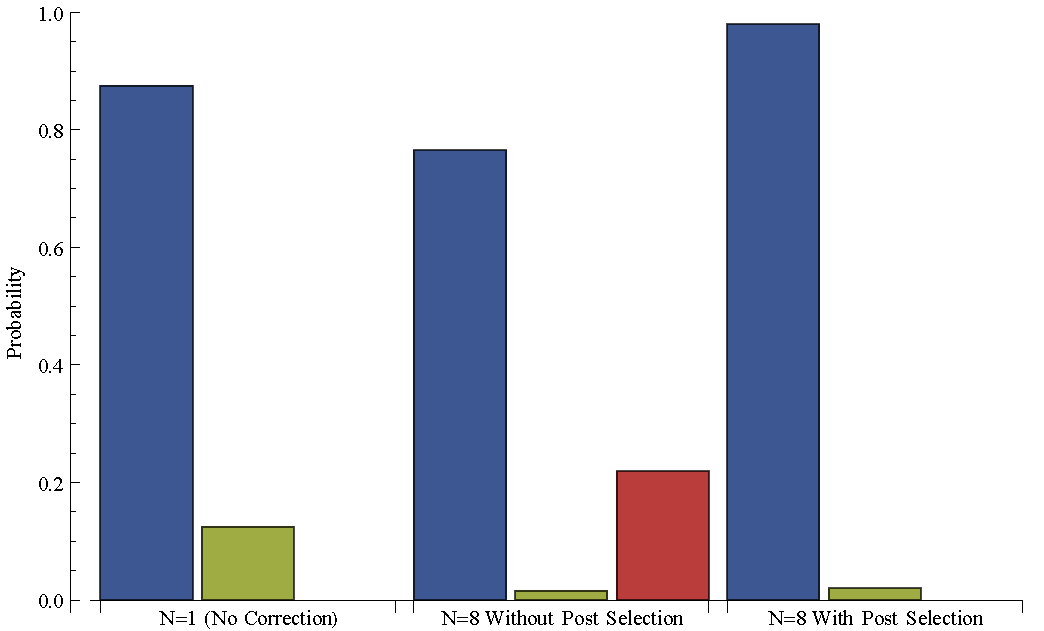
\includegraphics[width=\columnwidth]{prob_distributions.pdf}
	\end{centering}
	\caption[Comparison of output probability distributions with and without Error Averaging.]{Comparison of output probability distributions with and without error averaging. N corresponds the the number of redundant copies of the unitary being employed. Here the effect post selection has on the output distribution can be seen. The blue bars represent the probability of observing the photon in the correct output mode, green corresponds to observing the photon in the incorrect output mode and red corresponds to observing the photon in any of the error detection modes. The probabilities are based on a single photon in a Mach-Zehnder interferometer with an individual phase shifters variance $v=0.5\ \textrm{rad}^{2}$.} 
	\label{fig:output_probabilities}
\end{figure}
The central limit theorem applies to the individual matrix elements of the averaged transformation and hence their variance decreases as $\frac{1}{N}$.  The form of the average matrix and the distribution of the transformations on a finite number of averages depends on the details of the noise applied to the network encoding.  The results presented in this paper analyse these details showing conditions in which this technique may be of utility. 

The next section introduces the averaging scheme and some mathematical details that apply in the most general case which is followed by a comparison between conventional error correction and our proposed error correction in Section~\ref{Comparison with conventional error correction}. Section~\ref{implementation} includes numerous proof of principle examples which serve to highlight the effects of Error Averaging with a focus on the behaviour of the probability of success. Section~\ref{averaging at end vs step} studies two different ways of redundantly encoding a single mode phase shift and the effects of the different encodings on the resultant error and probability of success.  We then numerically analyse the averaging method for a four-mode operation in section~\ref{Four Mode Impementation Comparison}.  We will discuss some of the consequence of these results as well as future directions in Section~\ref{Discussion} before making some concluding remarks. 

% NOTATION SUGGESTION: Use \hat{} for Fock space operators and no hat for normal matricies.
\section{General Unitary Error Averaging\label{gen case}}

Here we are concerned with the case of bosonic linear scattering networks.  These are evolutions of a multi-mode bosonic field where the Heisenberg equations of motion for the annihilation operators of each mode can be written as a linear combination of all annihilation operators.  That is, if $\mathcal{U}_U$ is a unitary operation on a $m$ mode system, then
\begin{equation}
	\mathcal{U}_U a_i \mathcal{U}_U^\dagger = \sum_j U_{ij} a_j
\end{equation}
where, to preserve commutation relationships, $U$ must be a unitary matrix.  It is the network matrix $U$ that we will focus on.

Consider a linear network whose elements are those of a Discrete Fourier Transform (DFT).  That is, we have a Heisenberg style evolution between mode annihilation operators of the form
\begin{equation}
	a_{j,r} \rightarrow \frac{1}{\sqrt{N}} \sum_{k=0}^{N-1} \omega^{rk} a_{j,k}	
\end{equation}
where $\omega = e^{-i2\pi /N}$ and zero-indexing has been used, that is, $k=0$ corresponds to the first mode. The first subscript for the annihilation operator denotes the input mode and the second describes a quantity of redundancy $N$ which we explain shortly. 

We then act the $N$ copies of a target unitary $U$.  By this we mean that there is some variation between the copies but the intention was to implement the unitary $U$.  This can be described by the transformation
\begin{equation}
	a_{j,r} \rightarrow \sum_{l=0}^{m-1} (U_r)_{lj} a_{l,r}.
\end{equation}
where $N$ noisy copies of $U$ are made, denoted here as $U_1, U_2, \ldots, U_N$, where we assume an independent error model across the redundancies. 

After this the DFT matrix is applied again.  This results in the overall transformation
\begin{equation}
	a_{j,r} \rightarrow \frac{1}{N} 
	\sum_{l=0}^{m-1} \sum_{k,k^\prime=0}^{N-1}
	(U_{k^\prime})_{lj} \omega^{(r+k)k^\prime} a_{l,k}.
\end{equation}
We consider the case where all redundant modes are initialised in the vacuum state and post-select on the cases where no photons are present in the output of the redundant modes.  This means that we only need consider the parts of this transformation expression where the second subscript of the annihilation operator is zero.  In this case we have
\begin{equation}
	\label{sum_transformation}
	a_{j,0} \rightarrow \frac{1}{N}\sum_{l=0}^{m-1} \sum_{k^\prime=0}^{N-1}
	(U_{k^\prime})_{lj} a_{l,0} = \sum_{l=0}^{m-1} (M_N)_{lj} a_{l,0}
\end{equation}
where $M_N$ is a matrix defined by
\begin{equation}
	M_N = \frac{1}{N} \sum_k U_k.
\end{equation}
This matrix is then the effective linear network matrix for the post-selected system.  It includes information about the probability of success and so in general it will be not unitary.  The remainder of this paper is directed towards analysing the scenarios that arise from the multitude of choices for $U_k$ that form the expression.

For the main theorem of our work we consider a general linear network described by a unitary network matrix $U$ with any dimensionality. 

%Theorem~\ref{Theorem 1} below states that given access to $N$ linear networks $\{U_1,U_2,\ldots,U_N\}$ which are randomly distributed such that for all $i \in {1,\ldots,N}$, and given $U_{r,s}=\alpha_{r,s}e^{i\theta_{r,s}}$, $\langle \left(\theta_{i}\right)_{r,s} \rangle = \theta_{r,s}$, $\left|\left(\alpha_{i}\right)_{r,s}-\alpha_{r,s}\right|\ll1$ and $Var(U_i) = \sigma_i^2 < \infty$  the mean values of these unitaries approaches $c\times\hat{U}$, where $0\le c\le1$, in the same sense as the central limit theorem. By the central limit theorem we also see that the variance, $\sigma_{i}^{2}$, scales as $\frac{1}{N}$.

\begin{theorem}
\label{Theorem 1}
Given $N$ linear networks described by unitary matrices $\{U_1,U_2,\ldots,U_N\}$ that are random with independent and identically distributed statistics such that for all $i~\in~{1,\ldots,N}$, $\langle U_i \rangle = M$.  Then the random variable 
\begin{equation}
	\label{sum_unitary}
	M_{N}=\frac{1}{N}\sum_{i=1}^{N}U_{i}
\end{equation}
is a matrix with mean value $M$ and whose matrix elements have variance scaling as $O(1/N)$.
\end{theorem}

\begin{proof}\label{Proof 1}
Our aim in the proof is to use the central limit theorem.  Consider matrix element $r,s$ of $M_N$.  This is a random variable
\begin{equation}
	\left(M_N\right)_{rs} = \frac{1}{N} \sum_{i=1}^N \left(U_i\right)_{rs}.
\end{equation}
As the matrix elements $(U_i)_{rs}$ are constructed from unitary matrices, their magnitude is bounded by $1$.  Given this finite domain, the real and imaginary parts have maximum variance and covariance of $1$ (though these extremal values are not simultaneously achievable).  Given this bounded variance, we can use the central limit theorem to conclude that the matrix element $\left(M_N\right)_{rs}$ is a random variable with mean value $M_{rs}$.
The variance of the real or imaginary part of $(M_N)_{rs}$ is then upper bounded by $1/N$ as per the central limit theorem.
\end{proof}

The question now is what forms the mean average matrix $M$ as defined in Theorem \ref{Theorem 1}, can take. First we consider the trivial case where the unitary matrices are $1 \times 1$ dimensional.

\begin{corollary}
\label{Corollary 1}
	If each $\{U_1,\ldots,U_N\}$ are $1 \times 1$-dimensional, then $M$ is a complex number with magnitude $|M| \leq 1$.
\end{corollary}
\begin{proof}
	Write $U_k = e^{i \theta_k}$ where $p(\theta)$ is the probability density function for each of the angles $\theta_k$. From Theorem~\ref{Theorem 1} we need to compute the mean value 
	\begin{equation}
		M = \int^\pi_{-\pi} e^{i\theta} p(\theta) \mathrm{d}\theta. \label{eq:single parameter, single mode}
	\end{equation}
This is exactly the characteristic function of $p(\theta)$ evaluated at $1$.  The characteristic function is complex valued and has bounded magnitude of $1$, which is the desired result.
\end{proof}

By corollary~\ref{Corollary 1} it can be concluded that for the $1\times1$-dimensional case we can write $M=cU$ where $0 \leq c \leq 1$ and $U=e^{i\theta}$ has magnitude 1.  

% NOTE TO SELF(APL): Talk more about post-selection and M in this section
%Here we can identify the coefficient $c$ as the probability of success and as such, after post selection, the matrix $c\times U_{N}$ can be renormalised to a unitary matrix $U_{N}$ with $\lim_{N\rightarrow\infty}U_{N}=U$. 

Next consider higher dimensional matrices whose distribution is generated by a single parameter.  In this case, for any hermitian matrix $T$, which can be thought of as an infinitesimal generator from the $u(n)$ Lie algebra, we have
\begin{equation}
	M=\int e^{i\theta T}p(\theta)d\theta 
	\label{eq:single parameter, multi-mode}.
\end{equation}
We can make a change of variables in $\theta$ so that the distribution is changed to one that has mean zero
\begin{align}
	M&=\int e^{i(\mu + \theta^\prime)T} p(\mu + \theta^\prime) d\theta^\prime\\
	&= e^{i\mu T} \int e^{i\theta^\prime T} \bar{p}(\theta^\prime) d\theta^\prime \label{eq:seperating errors and transformations}
\end{align}
where $\bar{p}(\theta) = p(\mu + \theta)$ so that it has mean value zero.  By expanding the matrix exponential this expression can be written as
\begin{equation}
	M=\sum_n \frac{(iT)^n}{n!} \int \theta^n p(\theta) d\theta,
\end{equation}
which now relates to the moments of the underlying distribution in $\theta$. Assuming $p(\theta)$ were a Gaussian distribution with mean zero and variance $\sigma^2$ then we can write
\begin{equation}
	M = \sum_{n \in even} \frac{(iT)^n}{n!} (n-1)!! \sigma^n
\end{equation}
where $n!! = n(n-2)(n-4)\dots$ is the double factorial.  This series can be written back in the form of a matrix exponential, and by reintroducing the mean value we have
\begin{equation}
	M = e^{i\mu T} e^{-\frac{\sigma^2}{2} T^2}
\end{equation}
If $T^2=I$, which would be the case when choosing a Pauli matrix for $T$, then this expression would simplify to
\begin{equation}
M=Ue^{-\frac{\sigma^2}{2}}  \label{eq:Gaussian Psuccess}
\end{equation}
where $U$ is the unitary generated by the average parameter for $p(\theta)$.  The decaying exponential for the magnitude depends only on the variation in the distribution of $\theta$.

In the full parameter case, provided the target unitary $U$ again commutes with all errors a similar result can be found as discussed in corollary \ref{Corollary 2}.

\begin{corollary}
\label{Corollary 2}
If $\{U_1,\ldots,U_N\}$ are random $n$-dimensional unitaries such that $U_k = U exp\{i \sum_l \alpha_{kl} T_l\}$ with $n^2$ generators $T_l$ that are all hermitian and satisfy $T_l^2=I$, the parameters $\alpha_{kl}$ distributed independently with PDF $p_{l}(\alpha_l)$ which are all Gaussian with mean zero and small (but possibly different) variances so that all $U_k$ approximately commute with each other, then $M = c U$ where $0 < c < 1$ and $U$ is a unitary matrix.
\end{corollary}
\begin{proof}
We will extend the proof of Corollary~\ref{Corollary 1} to the $n$-dimensional case.  From the independence of the distributed parameters, we can write a PDF for all parameters as $p(\alpha_1,\ldots,\alpha_{n^{2}}) = p_1(\alpha_1)\times\ldots\times p_{n^2}(\alpha_{n^{2}})$.  
%For any Write where $T_l$ are generators of the $u(n)$ Lie-algebra of which there are $n^2$ and $U$ is chosen so that the distribution is defined by probability density function $p(\alpha_1,\ldots,\alpha_{n^{2}})$ has mean zero. $T_l$ are chosen so that and $-\pi < \alpha_l < \pi$. 
%As all errors are taken to be independent we can also write  
The approximate mutual commutivity for this expansion means 
\begin{widetext}
\newcommand{\theint}{\int^\pi_{-\pi} \ldots \int^\pi_{-\pi} \int^\pi_{-\pi}}
\newcommand{\theintd}{\mathrm{d}\alpha_1 \mathrm{d}\alpha_2 \ldots \mathrm{d}\alpha_{n^{2}}}
\begin{equation}
	\int^\pi_{-\pi} \int^\pi_{-\pi}
	[\alpha_{kl}T_{l},\alpha_{km}T_{m}] p_l(\alpha_l)p_m(\alpha_m) \mathrm{d}\alpha_l \mathrm{d}\alpha_m \approx 0 \quad \forall l,m,
\end{equation}
or in other words, that the $\alpha_{kl}T_l$ are all small with high probability.  With this we can write $M$ as
\begin{align}
	M &= U \theint
	exp\{i \sum_l \alpha_{l} T_l\} p_1(\alpha_1)\ldots p_{n^2}(\alpha_{n^{2}})
	\theintd
	\label{eq:general integral form} \\
	&\approx U \theint
	\prod_{l}exp\{i \alpha_{l} T_l\}p_1(\alpha_1)\ldots p_{n^2}(\alpha_{n^{2}})
	\theintd  \\
	&= U\int^\pi_{-\pi} exp\{i \alpha_{1} T_1\}p_1(\alpha_1) \mathrm{d}\alpha_1 	\int^\pi_{-\pi} exp\{i \alpha_{2} T_2\}p_2(\alpha_2) \mathrm{d}\alpha_2 \ldots \int^\pi_{-\pi}
	exp\{i \alpha_{n^2} T_{n^2}\}p_{n^2}(\alpha_{n^2}) \mathrm{d}\alpha_{n^2} \\
	&\approx U \prod_l e^{-\frac{\sigma_l^2 T_l^2}{2}},\label{eq:approx commuting, general case}
\end{align}
\end{widetext}
where $\sigma_l^2$ is the variance of $p_l$ and the final approximation is assuming the distribution is small so that the bounds of the integration do not matter.  Using the $T_l^2=I$ requirement on the generators the final product of exponentials can be identified with the value $c$, we have the desired result.
\end{proof}
The requirement of $T_L^2=I$ merely reflects a simplification where the generators are built from the Pauli matricies which are the constructions we will focus on in this paper.  If this is not the case then it is possible to identify the hermitian operator $\prod_l e^{-\frac{\sigma_l^2 T_l^2}{2}}$ as a state dependant decay in the amplitude of the operator.

%It should be noted that if the distribution of parameters is Gaussian but not indepenent, then there is gaurenteed to be a linear combination of parameters for which this distribution is indepdenant.  Hence by changing the generators in the apropraite way, one can always arrange this situation for Gaussian distributions of the parameters $\alpha_{kl}$.


%From Corollary \ref{Corollary 2} and given our previous result for a Gaussian error distribution we can conclude that
%\begin{equation}
%M = U\prod_{l}^{n^2}e^{-\frac{\sigma_{l}^{2}}{2}}\label{eq:approx commuting, general case}
%\end{equation}
%To be clear this results requires that the errors are small such that they approximately commute with one another and with the target matrix $U$. The distributions $p(\alpha_{l})$ are also, in general, not equivalent, even if each component within a system has an equivalent error distribution the beam splitter parameters will not necessarily corresponds directly to the coefficients of the generators in the Lie algebra. 

Finding expressions for the matrix $M$ outside of the situations just outlined is an open problem.  In the most general case, $M$ is not proportional to a unitary matrix.  Furthermore, is not guaranteed that $M$ will satisfy the conditions for a normal matrix and hence cannot be unitary diagonalised.  So it is unclear if in general this post-selected regime has any connection to unitary quantum evolution at all.  Nevertheless, we will begin to examine situations which approach this domain through decompositions into single parameter problems and using numerical computations.

\section{Comparison with conventional quantum error correction \label{Comparison with conventional error correction}}

It is insightful to qualitatively discuss the parallels between conventional qubit quantum error detection and correction techniques, and our error averaging technique. The simplest code to see this parallel is by considering the 3-qubit code, which is able to detect and correct at most a single physical bit-flip error on a 3-fold redundantly encoded logical qubit. In the 3-qubit code the logical qubit is encoded via GHZ-type entanglement across the three physical qubits using two maximally entangling CNOT gates. 
Specifically, encoding implements the redundant mapping $\alpha\ket{0} + \beta\ket{1} \to \alpha\ket{000} + \beta\ket{111}$ in the logical basis. In our scheme, on the other hand, the redundant encoding takes the form of W-like entanglement, implemented via an optical fanout operation, where a single excitation in a single mode is mapped to a superposition of a single excitation across multiple modes. Specifically, the encoding is of the form $\hat{a}_1^\dag \to \frac{1}{\sqrt{N}}(\hat{b}_1^\dag + \dots + \hat{b}_N^\dag)$. This is qualitatively very distinct from the previous GHZ-type encoding, since GHZ states are maximally-entangled states, whereas W-states are not. Unlike GHZ states, which collapse onto a perfectly mixed $N-1$ qubit state upon loss of just a single qubit, the loss of a single mode from a W-state preserves most entanglement for large $N$. This leads us to speculate that this property of W-states enables much of the structure of encoded states to be preserved upon localised errors. Indeed, for $N\gg 1$ we anticipate that the failure of a relatively small subset of the redundant operations will have little impact on the integrity of the entire encoded state, owing to this unique property of the structure of loss in W-states.

Like conventional quantum error correction, we observed error threshold behaviour in our analysis. That is, we are only able to improve the fidelity of a state if its initial fidelity is above an error correction threshold. Below this threshold the error correction technique fails to improve the state. Indeed, non-zero thresholds must necessarily apply so as not to violate the quantum no-cloning theorem.

We observed that a simple form of circuit concatenation, whereby the protocol is recursively embedded within itself to construct larger nested codes, enables higher degrees of error correction, asymptoting to some maximum. This is congruent with conventional codes, where code concatenation asymptotically improves error correction at the expense of increased physical resources to mediate the more complex encoding.

In our scheme the post-selection upon detecting no photons in the designated failure modes is equivalent to syndrome measurement in traditional qubit codes. Successful post-selection effectively projects the encoded state back into the codespace, whereas failure heralds an unsuccessful syndrome extraction, thereby mapping the unitary error to a located loss error. The probability of detecting no photons in the failure modes can be associated with the error detection probability in traditional codes, and the respective conditional probability of measuring the correct output state with the error correction probability.

An interesting open question is whether the structure of the redundant encoding we utilise in our protocol may be translated to other physical architectures or conventional qubit settings, or rather whether it is very specific to photonic linear optics.

\section{Implementation\label{implementation}}

This section demonstrates how Error Averaging can be implemented for various example optical systems. These examples also serve as a verification of the range of validity of the approximately commuting errors assumption. It can also be noted that Equation~(\ref{sum_unitary}) can become the appropriate transformation for duality quantum computing by allowing the $U_{i}$ to be arbitrary\cite{dualityQC}.

Constructions for the redundant encoding using the DFT implementation from the previous section are useful mathematically but may be inconvenient to implement in practice.  The transformation of Eq.~(\ref{sum_transformation}) can also be achieved using an array of beam-splitters as shown in Fig.~\ref{fig:gen system}.  This beam-splitter array has the desirable property of being generated by a recursive pattern.  As shown by the bounding rectangles in Fig.~\ref{fig:gen system}, the outer and inner layers share the same basic structure. 

\begin{figure}[tbh]
	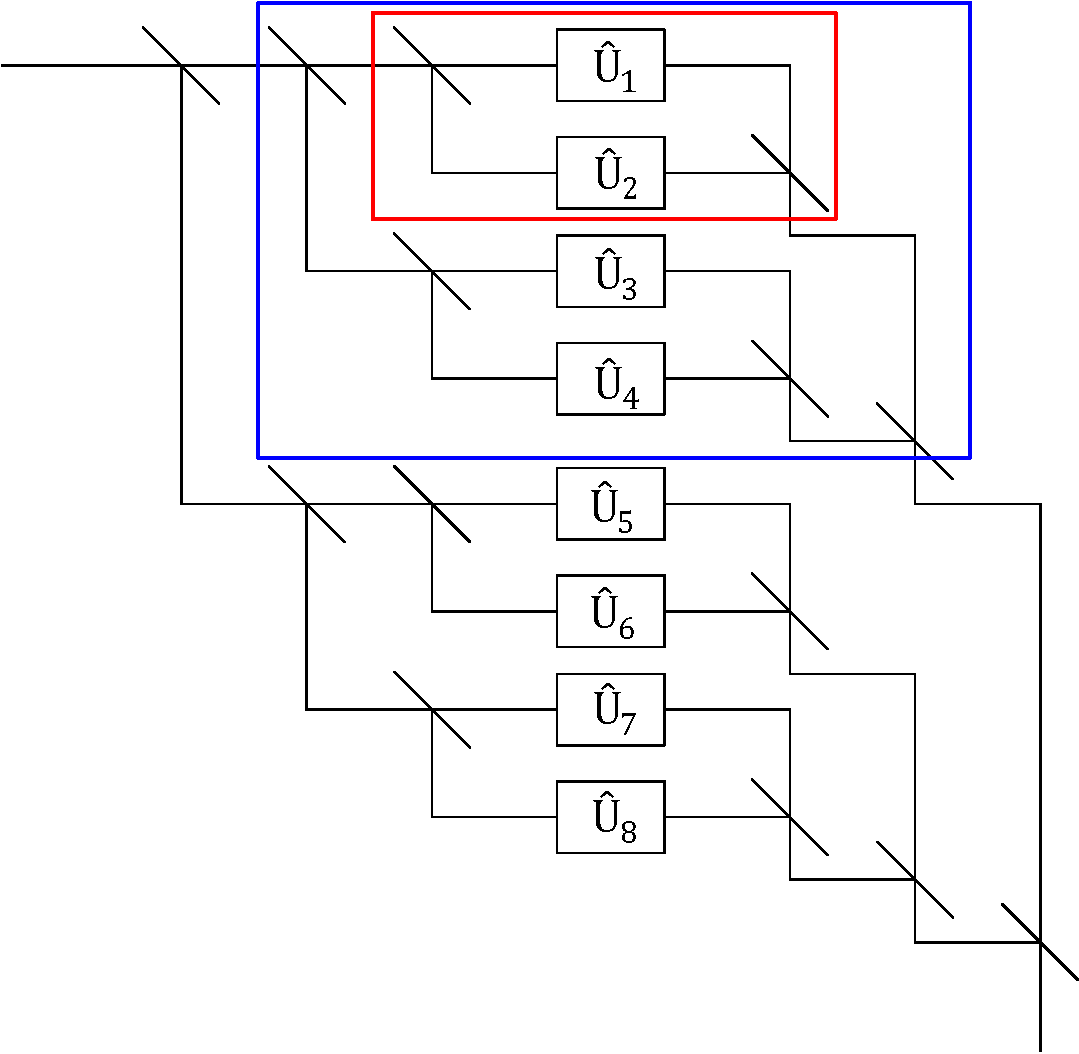
\includegraphics[width=\columnwidth]{unitaries.pdf}
	\caption{\label{fig:gen system}Redundant encoding using 50:50 beam-splitters for $N=8$. The boxes labelled $\hat{U}_i$ can be single or multi-mode.  In the multi-mode case the encoding beam-splitter network is repeated for each mode input and output. Output modes that are post-selected on the vacuum are not shown here. The red box shows an $N=2$ level encoding and the blue box shows $N=4$.  Further nesting of this arrangement can achieve any $N$ being a power of two.}
\end{figure}
	
%The following section discusses the results of numerical simulations for various systems implementing Error Averaging. To understand why linear optics was the chosen implementation consider the two key requirements of implementation. The first requirement is that the fundamental particle used as the computational qubit can be placed in a spacial superposition. The second requirement is that any employed unitary $\hat{U}$  does not act on the vacuum, that is $\hat{U}\left|0\right>=\left|0\right>$. Although these seem restrictive, LOQC automatically satisfies both of these requirements. A spacial superposition can be created easily using beam splitters and any linear optical unitary cannot, by definition, affect the vacuum.
	
%	Within the LOQC architecture, the following discussion will be agnostic about the specific encoding method by working in the Fock basis. In this way both single and dual rail encoding can be corrected and as such will generally not be considered in all further discussions.

%Initially we will focus on phase errors as this case is well understood and sets the stage for developing more complex scenarios.  The fundamental components in linear networks are phase shifters and beam splitters.  

All linear networks can be generated by arranging networks of beam-splitters and phase shifts~\cite{reck}.  Carolan et.~al.~\cite{ULO} have experimentally probed a linear network where all possible networks can be generated using controllable phase shifts and unvarying beam-splitters.  In their experimental implementation they demonstrated the ability to implement many quantum logic gates and linear optical protocols with a high fidelity.  Following this same methodology one can generate controllable beam-splitters using a Mach-Zehnder (MZ) interferometer consisting of a controllable phase shift in one arm and two fixed $50:50$ beam splitters.

Within this type of architecture the controllable phase shift is the key source of non-systematic noise.  Furthermore, redundantly encoding phase shifts are well characterised by the results presented above from Corollary~\ref{Corollary 1}.  So we will focus on phase shift induced errors for the analysis of this section and the next.  The model we will use assumes $50:50$ beam-splitters which are fixed and phase shifts that vary and are the source of all noise.

The noise in a controllable phase-shift can be written as $e^{i(\theta+\delta)}$ where $\theta$ is a real number representing the phase shift to be applied and $\delta$ is a zero-mean random variable representing the error.  For the identity operation $\theta=0$.  We will assume the distribution for $\delta$ to be Gaussian with variance $v$.  For values of $v$ that are comparable to $\pi^2$ the multi-valued nature of phase shifts becomes important.  But initially we will focus on the limit where $v \ll \pi^2$.

%In terms of the constructions used in Section~\ref{gen case}, this corresponds to Equation \ref{eq:single parameter, multi-mode} with $T=\begin{bmatrix}	0 & 1 \\	1 & 0 \\\end{bmatrix}$ and $M=e^{i\delta T}$ where we have set $U=\mathbb{I}$. 

%Need to come back to this.  Not sure what it means.

The remainder of this section considers the above implementation of a tunable beam-splitter as a MZ interferometer with the phase shift being error averaged. The error averaging will be performed using the concatenated beam-splitter network, hence $N=2^n, n \in \mathbb{N}$ and all beam-splitters used in this system will be fixed and with a splitting ratio of 50:50. We will analyse two key cases, the single photon and two photon performance.  The former involves the classical wave nature of the probability distribution for a single photon.  The latter includes Hong-Ou-Mandel~\cite{hom} style quantum interference.

\subsection{1 photon inputs \label{1 photon N arbitrary}}

The 1 photon network considered here is shown in Figure~\ref{fig:MZ_setup} both without any correction \ref{fig:uncorrected MZ beam splitter} and for the $N=2$ case \ref{fig:corrected MZ beam splitter}.  
\begin{figure}[tbh]
	\begin{subfigure}[b]{0.8\columnwidth}
		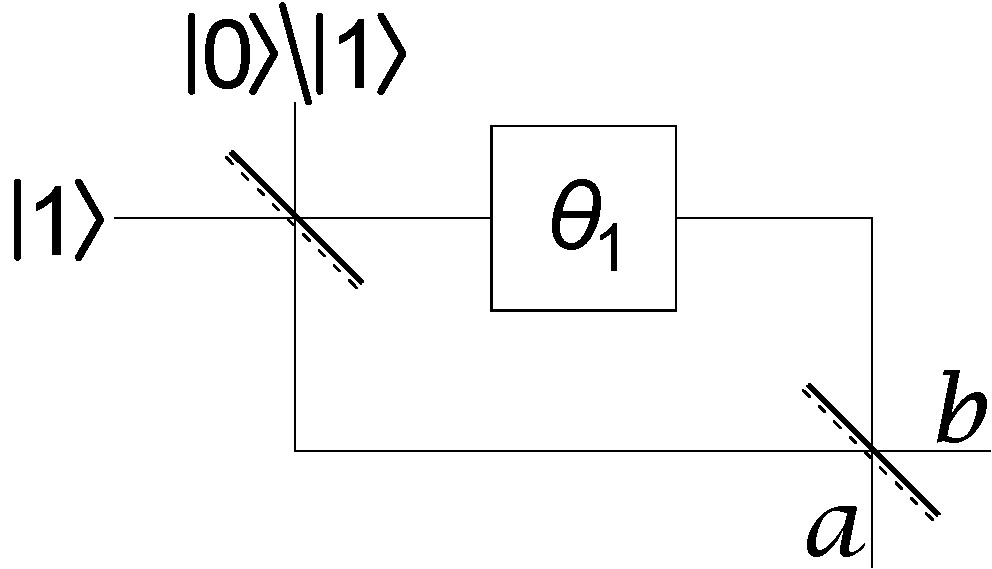
\includegraphics[width=1\columnwidth]{beam_splitter_system_a.pdf}
		\caption{}
		\label{fig:uncorrected MZ beam splitter} 
	\end{subfigure}
	
	\begin{subfigure}[b]{0.9\columnwidth}
		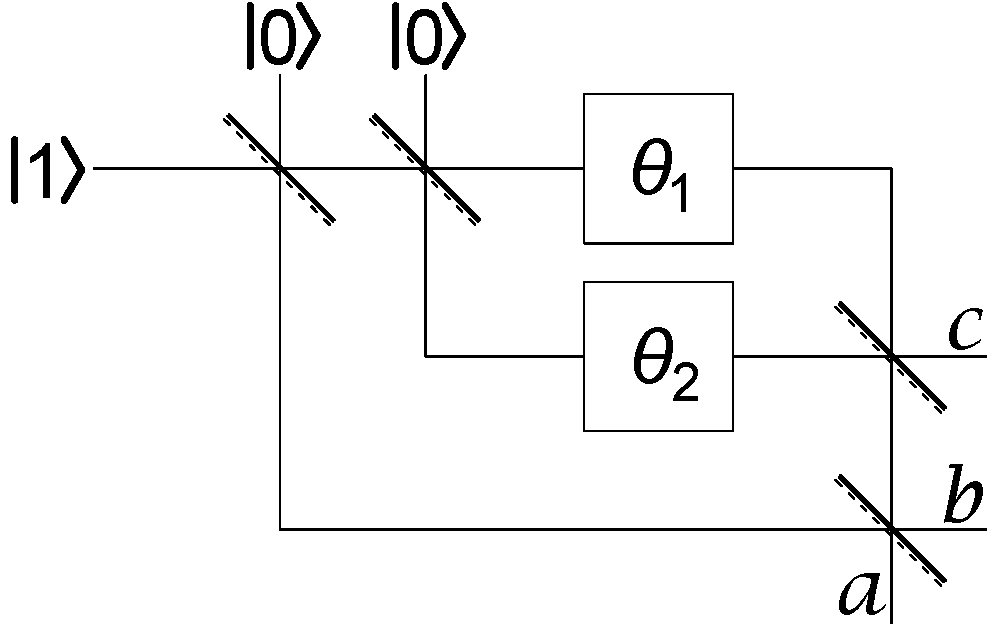
\includegraphics[width=\columnwidth]{beam_splitter_system_b.pdf}
		\caption{}
		\label{fig:corrected MZ beam splitter}
	\end{subfigure}
			\caption{\label{fig:MZ_setup}Diagram of MZ based tunable beam-splitter. (a) An uncorrected beam splitter implemented via MZ interferometer and (b) such a beam splitter corrected by redundantly encoding the phase shift, here for $N=2$. $a$ and $b$ label output modes and $c$ labels an error detection mode. The input state shown is used for both one and two photon calculations. The phase shift elements are marked with $\theta_{j}$ and are random variables.}
\end{figure}
	
The input single photon state is $\left|\phi\right\rangle = \hat{a}^{\dagger}\left|0\right\rangle $.  After traversing the error averaged network, the resulting un-normalised output state conditional on all encoded modes being vacuum is
\begin{multline}
	\ket{\psi} = \left(
	\left( \frac{e^{i\theta}}{2} \left\{\frac{1}{N}\sum_{j=1}^{N}e^{i\delta_{j}}\right\} + \frac{1}{2}\right) \hat{a}^{\dagger}  \right. \\
	+ \left. \left(\frac{e^{i\theta}}{2} \left\{\frac{1}{N}\sum_{j=1}^{N}e^{i\delta_{j}}\right\} - \frac{1}{2}\right) \hat{b}^{\dagger} 
	\right)
	\ket{0}.
	\label{eq:1ParbN}
\end{multline}
which is consistent with Theorem~\ref{Theorem 1}. Here $\theta_{j}=\theta+\delta_{j}$ with $\theta$ a constant and $\delta_j$ a random variable. 

As linear networks conserve photon number, and we have post-selected the cases where energy exits via the redundant encoding modes, we know that the output state always contains one and only one photon.  The probability that the photon is measured in a particular mode can therefore be equated to the average photon number in that mode.  Using this we can calculate from the un-normalised state $\ket{\psi}$ the probability of observing the photon in the $\hat{a}$ and $\hat{b}$ modes without post-selection to be 
\begin{eqnarray}
	\bra{\psi} \hat{a}^{\dagger}\hat{a} \ket{\psi} & \approx & \cos^{2}\left(\theta/2\right)+\frac{v}{4N}-\frac{v\cos^{2}(\theta/2)}{2}
\end{eqnarray}
and
\begin{eqnarray}
	\left\langle \psi\right|\hat{b}^{\dagger}\hat{b}\left|\psi\right\rangle & \approx & \sin^{2}\left(\theta/2\right)+\frac{v}{4N}-\frac{v\sin^{2}(\theta/2)}{2}
\end{eqnarray}
where we have taken a first-order expansion in the phase shift variance $v$.
The probability of success is the sum of the probabilities of the $\hat{a}$ mode and $\hat{b}$ mode.  This is 
\begin{eqnarray}
	P(\textrm{success}) & = & \bra{\psi}\hat{a}^{\dagger}\hat{a}\ket{\psi} +\bra{\psi}\hat{b}^{\dagger}\hat{b}\ket{\psi} \\
	& \approx & 1+\frac{v}{2N}-\frac{v}{2}. \label{eq:1pNarbitrary successs}
\end{eqnarray}
In the large $N$ limit, this corresponds to the linear approximation of Equation \ref{eq:Gaussian Psuccess} where we can identify $P(\textrm{success})=c$. 

Without any noise, choosing $\theta=0$ results in complete interference and the input single photon state will be transferred to a single output.  Any deviations from this are attributed to non-ideal interferometer performance. 
In this case the probability of observing the output in the correct mode without post-selection is
\begin{equation}
	\left\langle \psi\right|\hat{a}^{\dagger}\hat{a}\left|\psi\right\rangle \approx 1 - \frac{(2N-1)v}{4N}. \label{eq:1pNoPost}
\end{equation}
After post-selection this becomes
\begin{equation}
	\frac{\left\langle \psi\right|\hat{a}^{\dagger}\hat{a}\left|\psi\right\rangle}{P(\textrm{success})} \approx 1 - \frac{v}{4N}. \label{eq:1pWithPost}
\end{equation}
		
Figure~\ref{fig:post vs no post} shows how these two quantities scale with $N$. In particular, it can be seen that after post-selection the likelihood of the photon exiting the interferometer in the correct mode can be made arbitrarily close to unity by increasing $N$. Also, while the probability of success decreases for increasing $N$ it asymptotes to a constant value. This implies that as $N$ increases, even though the total quantity of errors added to the system increases, the effects of the combined errors on the interferometer is less. This result is also not dependent on the value chosen for $\theta$. Explicitly as the intended phase shift can be factored out in Eq. \ref{eq:1ParbN} similarly to the result shown in Eq. \ref{eq:Gaussian Psuccess} the effects of errors and our error correction can be considered separately from the transformation being applied.
%This can be understood as the process of redundantly splitting and recombining the state, driving noise into the post-selected ports by interference.  
\begin{figure}[tbh]
	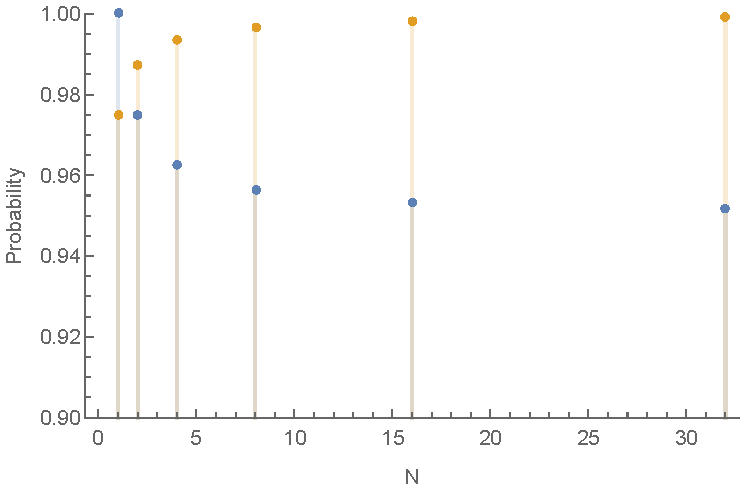
\includegraphics[width=\columnwidth]{1photonpostvsnopost.pdf}
	\caption{\label{fig:post vs no post} Probability of single photon being detected at the $a$ output port as shown in Figure~\ref{fig:MZ_setup} as a function of the redundant encoding size $N=2^n$. Here the phase shifts are sampled from a distribution with mean value $0$ and variance $v=0.1\ \textrm{rad}^{2}$. The blue values give the probability of success and the orange values corresponds to the probability of obtaining the correct result conditional on the photon not exiting the added redundant encoding modes, that is, with post-selection.  Eq.~(\ref{eq:1pNarbitrary successs}) predicts an asymptote of $0.95$ without post-selection and Eq.~(\ref{eq:1pWithPost}) predicts an asymptote of $1$ with post-selection.  The asymptotic behaviour is consistent with the plotted data.}
\end{figure}

\subsection{2 photon inputs\label{2 photons N arbitrary}}

The single photon interference effects in linear networks can be explained using classical wave interference.  Now we will consider two photon interference to demonstrate the behaviour of quantum interference when using the redundant encoding. As such here $\left|1,1\right\rangle$ is used as the input state. Again, a diagram of the explicit set-up with and without the redundant encoding can be seen in Figure \ref{fig:MZ_setup}. For two photons the un-normalised output state for the $a$ and $b$ modes is
\begin{multline}
	\ket{\psi} =  \frac{1}{2}\left\{ 1+\frac{1}{N^{2}}\left(\sum_{j=1}^{N}\sum_{k=1}^{N}e^{i(\delta_{j}+\delta_{k})}\right)\right\} \ket{1,1} \\
	+\frac{\sqrt{2}}{4}\left\{ \frac{1}{N^{2}}\left(\sum_{j=1}^{N}\sum_{k=1}^{N}e^{i(\delta_{j}+\delta_{k})}\right)-1\right\} \left(\ket{2,0} +\ket{0,2}\right)\label{eq:2pNarbitrary S}
\end{multline}
where we have chosen $\theta=0$ when computing this state. This is done, as above, to simplify the form of the equations and does not change the effect of the redundant encoding on the errors.  Because of this choice, the action of the interferometer on the input state should be the identity operation and hence $\ket{1,1}$ is the desired output state.   Note that we could have chosen the input state to be $\ket{2,0}$, but this would not necessarily show any new behaviour, just the single photon results independently applied to the two input photons. 

We can again write probabilities as expectation values of occupation number.  Using the form of Eq.~(\ref{eq:2pNarbitrary S}), the ideal output is achieved when
\begin{equation}
\bra{\psi}\hat{a}^{\dagger}\hat{a}\hat{b}^{\dagger}\hat{b}\ket{\psi} = 1.
\end{equation}
This expectation value for the state including the phase shift noise is
\begin{eqnarray}
\left\langle \psi\right|\hat{a}^{\dagger}\hat{a}\hat{b}^{\dagger}\hat{b}\left|\psi\right\rangle & = & \left\langle \left|\frac{1}{2}\left\{ 1+\frac{1}{N^{2}}\left(\sum_{j=1}^{N}\sum_{k=1}^{N}e^{i(\delta_{j}+\delta_{k})}\right)\right\} \right|^{2}\right\rangle \nonumber \\
& = & \left\langle \frac{1}{4}\left(1+\frac{2}{N^{2}}\left(\sum_{j=1}^{N}\sum_{k=1}^{N}\cos\left(\delta_{j}+\delta_{k}\right)\right)\right)\right\rangle \nonumber \\
&  & +\frac{1}{4}\Biggl\langle\frac{1}{N^{4}}\left(\sum_{j}^{N}e^{-2i\delta_{j}}+\sum_{j=1}^{N}\sum_{k\ne j}^{N}e^{-i(\delta_{j}+\delta_{k})}\right)\nonumber \\
&  & \times\left(\sum_{l}^{N}e^{2i\delta_{l}}+\sum_{l=1}^{N}\sum_{m\ne l}^{N}e^{i(\delta_{l}+\delta_{m})}\right)\Biggr\rangle\nonumber \\
& \approx & 1-v\label{eq:exp. value aabb}
\end{eqnarray}
where the approximation is assuming $v$ small.  Post-selection will increase this to 
\begin{widetext}
\begin{eqnarray}
P(\textrm{coincidence}) & = & \frac{\left\langle \psi\right|\hat{a}^{\dagger}\hat{a}\hat{b}^{\dagger}\hat{b}\left|\psi\right\rangle }{\left\langle \psi\right|\hat{a}^{\dagger}\hat{a}\hat{b}^{\dagger}\hat{b}\left|\psi\right\rangle +0.5\left\langle \psi\right|\hat{a}^{\dagger}\hat{a}^{\dagger}\hat{a}\hat{a}\left|\psi\right\rangle +0.5\left\langle \psi\right|\hat{b}^{\dagger}\hat{b}^{\dagger}\hat{b}\hat{b}\left|\psi\right\rangle }\nonumber \\
& \approx & 1-\frac{v}{2N}\label{eq:2pNarb PS}
\end{eqnarray}
\end{widetext}
where $P(\textrm{coincidence})$ is the probability the photons exit modes $a$ and $b$ individually and the binomial approximation has been used to keep only variance terms to first order.  Finally the probability of success, which is the probability no photons exit the encoding modes is 
\begin{eqnarray}
	P(\textrm{success}) & \approx & 1-v+\frac{v}{2N}.\label{eq:2pNarb Success}
\end{eqnarray}
Again, the large $N$ limit of this equation the result matches the prediction of Equation~\ref{eq:Gaussian Psuccess}. Also, the probability of success has a $\frac{1}{N}$ scaling which is the same as for the single photon input case. 

In this section we have demonstrated how redundantly encoding variable components can reduce the resulting variance within a system for the simple but highly important case of a single beam splitter. We have also shown that the results match what is expected from the couple of solved exact cases discussed in Section \ref{gen case}. In the following section we will give some more complex examples to give a clearer insight into how this redundant encoding might best be applied, and its effect in the situations where the mathematical machinery introduced earlier is not easily solvable.

\section{Comparison between averaging techniques \label{averaging at end vs step}}

In this section we will study two different methods, which we will refer to as \textit{averaging at the end} and \textit{averaging each step}. To illustrate the two approaches we consider a simple system of phase-shifters. Fig.~\ref{fig:Different methods of implementation} shows schematically these two configurations as well as a baseline comparison. The system analysed is applying a single mode phase-shift generated by $M$ sequential phase shifters.  Averaging across the entire system applies the $M$ phases and redundantly encoding this $N$ times (Figure~\ref{fig:Different methods of implementation b}). The method of averaging each step involves a redundancy of $N$ for each of the $M$ applied phase shifts (Figure~\ref{fig:Different methods of implementation c}).  When averaging each component individually significantly more encoding beam-splitters are required, however we will show this leads to more stability in the output state for larger errors. In the low error limit however these two methods yield equivalent results. Because of this the difference in clearer when results are taken to the the higher order and as such in the following section all approximations will be taken to the second order in the variance as opposed to the first order as done above.

\begin{figure}
	\centering
	\begin{subfigure}[b]{\columnwidth}
		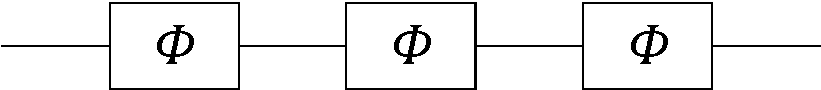
\includegraphics[width=0.65\columnwidth]{three_phase_applying_systems_a.pdf}
		\caption{}
		\label{fig:Different methods of implementation a} 
	\end{subfigure}
	
	\begin{subfigure}[b]{\columnwidth}
		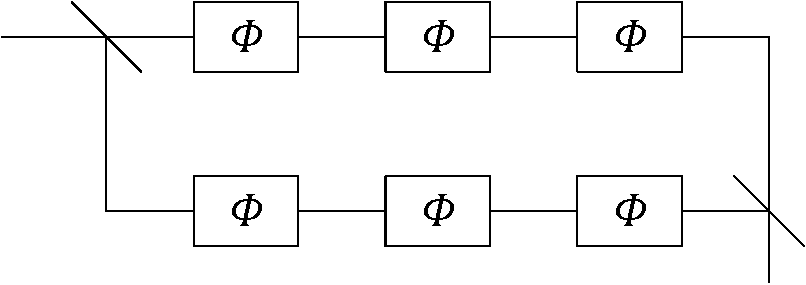
\includegraphics[width=0.80\columnwidth]{three_phase_applying_systems_b.pdf}
		\caption{}
		\label{fig:Different methods of implementation b}
	\end{subfigure}

	\begin{subfigure}[b]{\columnwidth}
		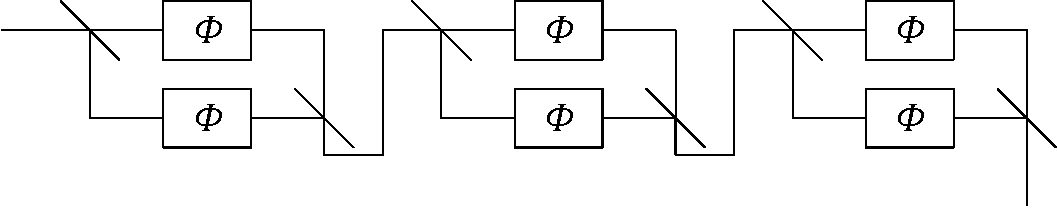
\includegraphics[width=1\columnwidth]{three_phase_applying_systems_c.pdf}
		\caption{}
		\label{fig:Different methods of implementation c}
	\end{subfigure}
	
	\caption[Two numerical solutions]{Three methods of applying three phase shifts, each marked with a in
			series. (a) Three phase shifts with no error averaging. (b) Three phase
			shifts when averaging across the system. (c) Three phase shifts when
			averaging across each phase shifter individually. Averaging across the
			system will in general require far fewer encoding resources.
			\label{fig:Different methods of implementation}}
\end{figure}
%\subsection{Single Mode, Single Parameter Examples \label{Phase applying systems}}

Following an approach motivated by the previous section the applied phase shifters were placed in one arm of a MZ interferometer. The applied phase shift was chosen to have mean zero with a Gaussian random noise with a variance $v$. This choice allows for the errors here to be compared with those modelled in sections~\ref{1 photon N arbitrary} and~\ref{2 photons N arbitrary}. The probability of success is now defined as the photon number expectation value evaluated at the end of the phase applying systems while the strength of the error is defined as the photon number expectation value of the MZ interferometer system at the expected output given no photon exited any of the redundant encoding modes. 

%All approximate results are based of fourth order Taylor approximations with comparisons drawn to the second order approximations as used in previous sections.

\subsection{No Averaging\label{No Averaging}}

Starting with the baseline comparison case where no Error Averaging is used (Fig.~\ref{fig:Different methods of implementation}(a)), the output state for a single photon going through $M$ phase shifters will be
\begin{equation}
\left|\psi\right\rangle =\left(\prod_{k=1}^{M}e^{i\delta_{k}}\right)\left|1\right\rangle \label{eq:noAvPhaseState}
\end{equation}
As there is no path for the photon to exit the system, the probability of success is always $1$.

To quantify the error the phase applying system it was then inserted into a MZ interferometer giving a total output state $\ket{\Psi}$.  As the mean phase shift is zero, the error is manifest in the photon expectation value at the correct output mode after post-selection. As however the probability of success is $1$ no post selection occurs here.  The output state from the MZ interferometer is
\begin{equation}
	\ket{\Psi} =\frac{1}{2}\left(\prod_{k=1}^{M}e^{i\delta_{k}}+1\right)\hat{a}^{\dagger}\ket{0}+\left(\prod_{k=1}^{M}e^{i\delta_{k}}-1\right)\hat{b}^{\dagger}\ket{0}. \label{eq:noAveIntState}
\end{equation}
The measure to the quantity of error which was used to compare the three situations chosen is the probability of observing the correct result conditional on the photon not being detected in an error mode, or $P(\textrm{correct})$. For no averaging this is
\begin{eqnarray}
P(\textrm{correct}) & = & \left\langle \Psi\right|\hat{n}_{a}\left|\Psi\right\rangle \nonumber \\
& = & \frac{1}{2}\left\langle 1+\cos\left(\alpha\right)\right\rangle \nonumber \\
& \approx & 1-\frac{Mv}{4}+\frac{M^{2}v^{2}}{16}\label{eq:ErrorNoAv1}
\end{eqnarray}
where $\alpha=\sum_{k=1}^{M}\delta_{k}$ and Gaussian statistics have been used to write higher order moments in terms of the variance.

\subsection{Averaging Across the Entire Phase System\label{Averaging Across the Entire Phase System}}

We now consider averaging across the whole system, as shown in Figure~\ref{fig:Different methods of implementation}(b). Proceeding as before, the state for a single photon after passing through $M$ phase shifters in series which is being averaged across $N$ times will simply be
\begin{equation}
	\ket{\psi}=\frac{1}{N}\sum_{j=1}^{N}\left(\prod_{k=1}^{M}e^{i\delta_{j,k}}\right)\ket{1} \label{eq:AvEndPhaseState}
\end{equation}
The probability of success is thus
\begin{eqnarray}
	P\left(success\right) & = & \braket{\psi|\psi} \nonumber \\
& \approx & \left[1-\left(1-\frac{1}{N}\right)\left(Mv-\frac{1}{2}M^{2}v^{2}\right)\right]\label{eq:AveEndProbSuccess}
\end{eqnarray}
This result is similar to the what was found in previous sections, see Eq.\ref{eq:1pNarbitrary successs} and Eq.\ref{eq:2pNarb Success}, with the probability of success asymptotically approaching some fixed value for large $N$.

To determine the size of the error, the phase applying system was again inserted into one arm of a MZ interferometer giving a total output state $\ket{\Psi}$. The error is then given by the photon expectation value in the correct output mode with post selection. The output state is
\begin{eqnarray}
	\ket{\Psi}& = &\frac{1}{2}\left(\frac{1}{N}\sum_{j=1}^{N}\left(\prod_{k=1}^{M}e^{i\delta_{j,k}}\right)+1\right)\hat{a}^{\dagger}\ket{0}\\ & & +\left(\frac{1}{N}\sum_{j=1}^{N}\left(\prod_{k=1}^{M}e^{i\delta_{j,k}}\right)-1\right)\hat{b}^{\dagger}\ket{0}\label{eq:AveEndIntState}
\end{eqnarray}
So the photon number expectation value for the expected output from the interferometer will be
\begin{widetext}
\begin{eqnarray}
	\bra{\Psi}\hat{n}_{a}\ket{\Psi}
& \approx & 1-\frac{1}{4}\left(Mv-\frac{M^{2}v^{2}}{4}+\left(1-\frac{1}{N}\right)\left(Mv-\frac{1}{2}M^{2}v^{2}\right)\right)
\end{eqnarray}
Similarly for the incorrect output port, the photon number expectation value will be
\begin{equation}
	\bra{\Psi}\hat{n}_{b}\ket{\Psi} = \frac{1}{4}\left\langle 1+\left\langle \psi|\psi\right\rangle -\frac{2}{N}\sum_{j=1}^{N}\cos\left(\alpha_{j}\right)\right\rangle 
\end{equation}
Therefore, our error measure, the conditional probability of observing the correct result, will now be
\begin{equation}
P(\textrm{correct})  \approx  \left[1-\frac{1}{4}\left(Mv-\frac{M^{2}v^{2}}{4}+\left(1-\frac{1}{N}\right)\left(Mv-\frac{1}{2}M^{2}v^{2}\right)\right)\right]\nonumber\times\left[1-\left(1-\frac{1}{N}\right)\left(\frac{Mv}{2}-\frac{1}{4}M^{2}v^{2}\right)\right]^{-1}\label{eq:ErrorAvEnd}
\end{equation}
\end{widetext}

\subsection{Averaging Across Each Phase Shifter Individually\label{Averaging Across Each Phase Shifter Individually}}

If each phase shifter is averaged individually, as seen in Figure \ref{fig:Different methods of implementation}(c), then the state for a single photon after passing through the phase applying system will be
\begin{equation}
	\ket{\psi}=\frac{1}{N}\prod_{k=1}^{M}\left(\sum_{j=1}^{N}e^{i\delta_{j,k}}\right)\ket{1}\label{eq:AveStepPhaseState}
\end{equation}
Reproducing the above calculations with this state yields a probability of success of
\begin{equation}
P\left(Success\right)\approx\left(1-\left(v-\frac{v^{2}}{2}\right)\left(1-\frac{1}{N}\right)\right)^{M}\label{eq:AvStepProbSuccess}
\end{equation}
and a conditional probability of observing the correct result of
\begin{widetext}
\begin{equation}
P(\textrm{correct}) \approx  \left[\frac{3}{4}-\frac{Mv}{4}+\frac{M^{2}v^{2}}{16}+\frac{1}{4}\left(1-\left(v-\frac{v^{2}}{2}\right)\left(1-\frac{1}{N}\right)\right)^{M}\right]\nonumber\times\left[\frac{1}{2}+\frac{1}{2}\left(1-\left(v-\frac{v^{2}}{2}\right)\left(1-\frac{1}{N}\right)\right)^{M}\right]^{-1}\label{eq:ErrorAvStep}
\end{equation}
\end{widetext}
Importantly, for both this case as well as when averaging each step, if only the first order approximation is used and $M=1$ then the error matches the error found in section \ref{1 photon N arbitrary}. However we see that with the second order terms included the two results diverge from one another. This can be seen most clearly in Figure \ref{fig:Probability-of-success all}.

\subsection{Summary of Errors and Probabilities\label{Summary of Errors and Probabilities}}

\begin{figure}
	\centering
	\begin{subfigure}[b]{\columnwidth}
		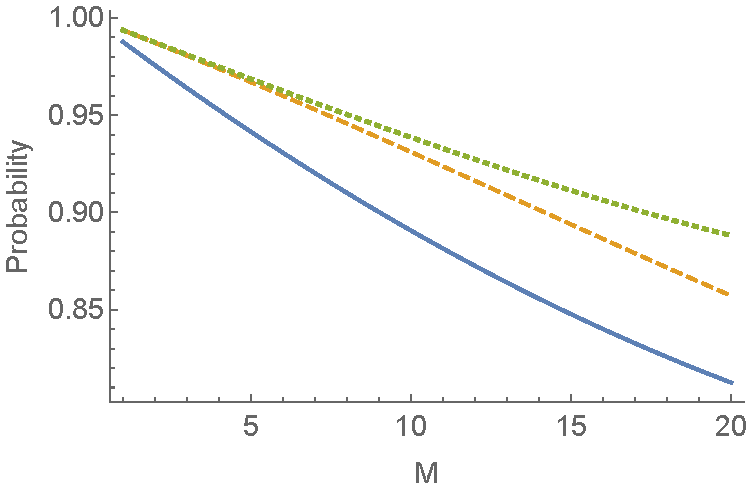
\includegraphics[width=1\columnwidth]{error_a.pdf}
		\caption{}
		\label{fig:Prob correct for phase systems a} 
	\end{subfigure}
	
	\begin{subfigure}[b]{\columnwidth}
		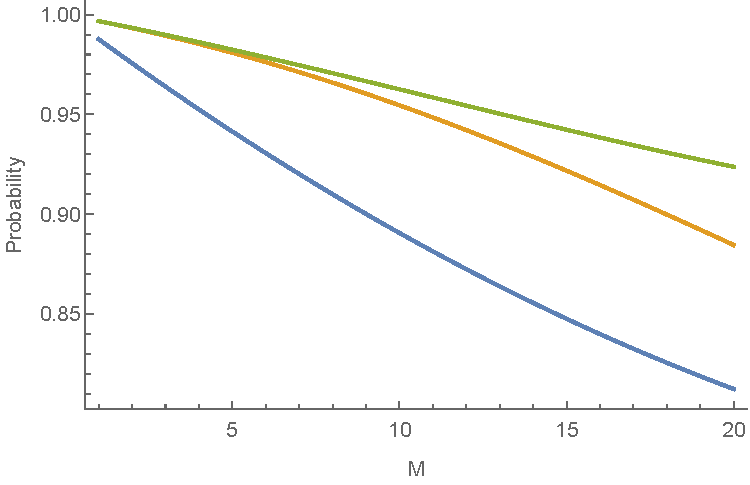
\includegraphics[width=1\columnwidth]{error_b.pdf}
		\caption{}
		\label{fig:Prob correct for phase systems b}
	\end{subfigure}
	
	\begin{subfigure}[b]{\columnwidth}
		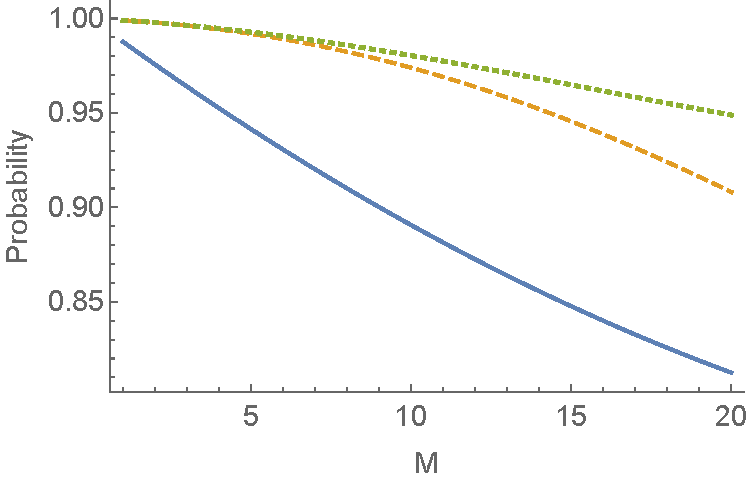
\includegraphics[width=1\columnwidth]{error_c.pdf}
		\caption{}
		\label{fig:Prob correct for phase systems c}
	\end{subfigure}
	
	\caption[Prob correct for phase systems]{Probability of obtaining the correct result as measured by the Mach-Zehnder interferometer set up as a function of the number of phase components $M$. Here a probability of $1$ corresponds to no error and the smaller the probability the larger the error. The blue line represents the no Error Averaging applied result, the orange line corresponds to the error when averaging across the entire system and the green line is the error when each component is averaged across individually. All three graphs were created with the variance of the error in a single phase shifter being $0.005\ \textrm{rad}^{2}$ and for (a) $N=2$, in (b) $N=4$ and in (c) $N=16$. \label{fig:Error-as-measured all}}
\end{figure}
%
Figure~\ref{fig:Error-as-measured all} shows how the error, as measured by looking at expected photon number values in the output port of a MZ interferometer, varies as the number of phase components increases as well as how the error changes with increasing Error Averaging, $N$. The behaviour as $N$ increases is as expected with the error close to disappearing for low $M$, that is, a small number of phase shifters in series, and $N=16$. Interestingly a difference between the two Error Averaging methods can be seen from $M\approx6$ onwards. This could either be suggesting an issue with the quality of the second order approximations, as seen in Figure~\ref{fig:Probability-of-success all} or that there is some more fundamental point at which there is a clear benefit to averaging each component individually. The next consideration was how the probability of success changes with $M$.

Figure~\ref{fig:Probability-of-success all} shows how the probability of success changes as the number of phase shifters in a series increases when averaging across the entire system as well as when averaging across each component individually. The effect of varying the amount of averaging is also shown for both the first and second order analytical solution. The top four graphs were plotted for a low value of the variance on the individual phase shifters. This was done so that the behaviour when the first and second order approximations diverge can be clearly seen. 

As the total number of components increases with both increasing $M$ and $N$, the probability of success decreases. However it does so at a decreasing rate which is important for scaling to large systems. The two methods of Error Averaging also show very similar behaviour in their overall trends although the variation between the first and second order approximations in the two encoding methods diverges. This is suggestive of a manifestation of the Zeno effect, whereby continuously correcting produces less variation than doing the same amount of correction at the end. First and second order solutions in the averaging over the entire system case diverge very early when compared with those for averaging every step. Interestingly it appears that the first order analytical approximation is suitable when averaging each component individually even for larger or equivalently higher error systems. This can most clearly be seen in Figure~\ref{fig:phase psuccess e} where the first order approximation diverges from the second order approximation almost instantly while in Figure~\ref{fig:phase psuccess f} the first and second order approximations both follow each other closely. It is again observed that as $N$ increases, the probability of success goes down. This could also be suggesting that the variation in the statistical simulation is also reduced, implying a greater amount of averaging reduces the variability in any given sample of the applied phase.
%
\begin{figure}
	\centering
	
	\begin{subfigure}[b]{.45\columnwidth}
		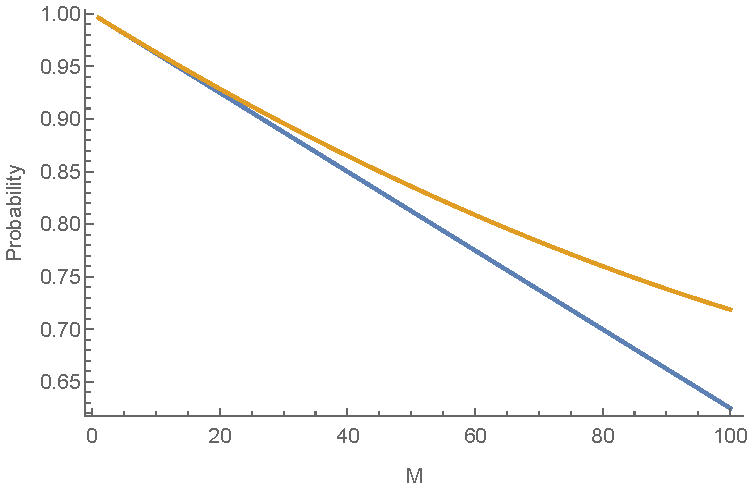
\includegraphics[width=\columnwidth]{Psuccess_a.pdf}
		\caption{}\label{fig:phase psuccess a}
	\end{subfigure}
	\begin{subfigure}[b]{.45\columnwidth}
		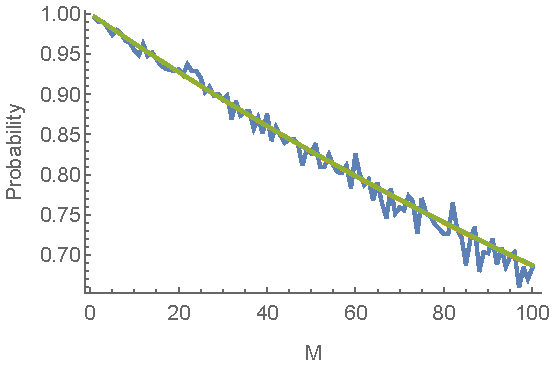
\includegraphics[width=\columnwidth]{Psuccess_b.pdf}
		\caption{}\label{fig:phase psuccess b}
	\end{subfigure}

	\begin{subfigure}[b]{.45\columnwidth}
		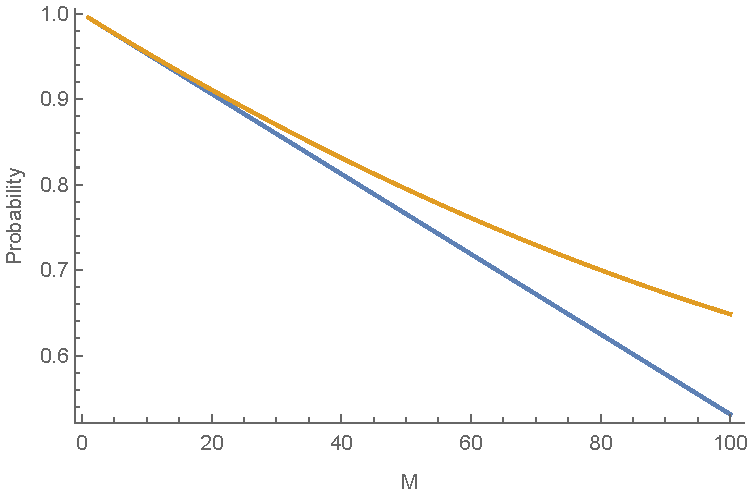
\includegraphics[width=\columnwidth]{Psuccess_c.pdf}
		\caption{}\label{fig:phase psuccess c}
	\end{subfigure}
	\begin{subfigure}[b]{.45\columnwidth}
		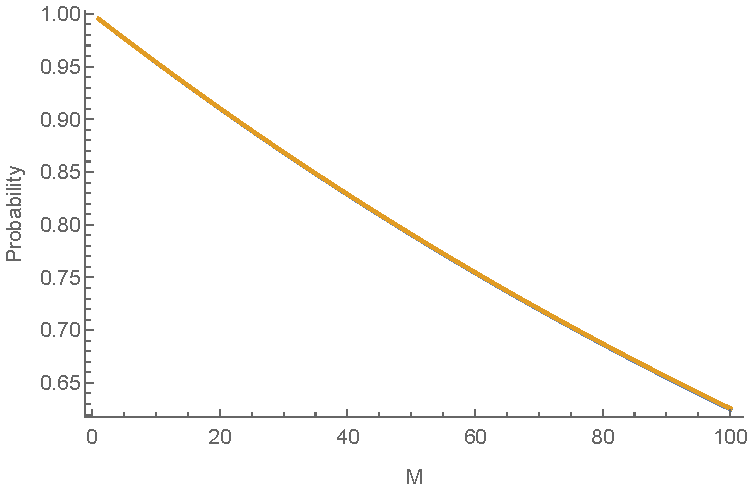
\includegraphics[width=\columnwidth]{Psuccess_d.pdf}
		\caption{}\label{fig:phase psuccess d}
	\end{subfigure}

	\begin{subfigure}[b]{.45\columnwidth}
		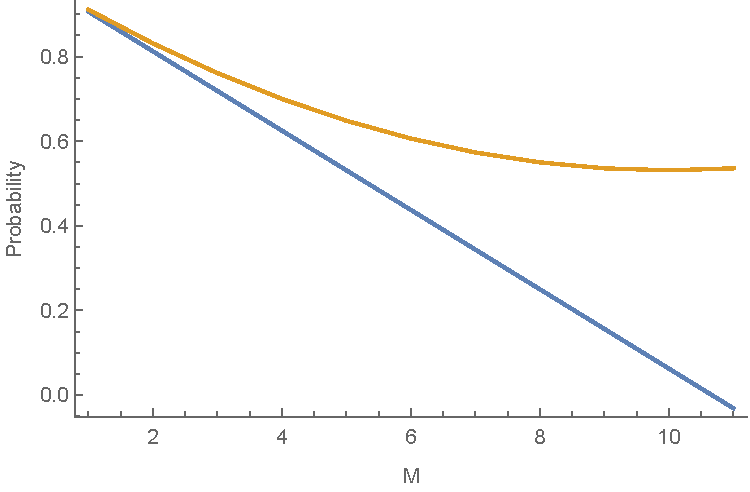
\includegraphics[width=\columnwidth]{Psuccess_e.pdf}
		\caption{}\label{fig:phase psuccess e}
	\end{subfigure}
	\begin{subfigure}[b]{.45\columnwidth}
		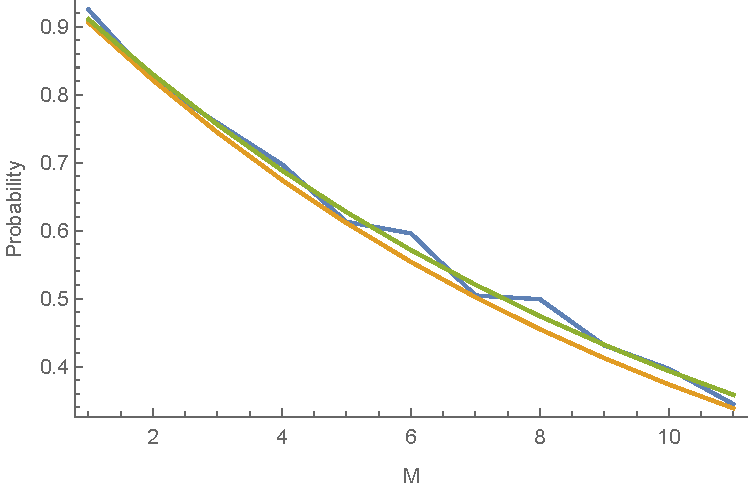
\includegraphics[width=\columnwidth]{Psuccess_f.pdf}
		\caption{}\label{fig:phase psuccess f}
	\end{subfigure}
	
	\caption[Prob success for phase systems]{Probability of success as a function of the number of phase components $M$ for averaging across the system (left) and averaging across each component (right). The blue line is the first order approximation and orange is the second order approximation of the analytical value. a) and b) individual phase shifter variance is $0.005\ \textrm{rad}^{2}$ with $N=4$, c) and d) individual phase shifter variance is $0.005\ \textrm{rad}^{2}$ with $N=16$ and e) and f) individual phase shifter variance is $0.1\ \textrm{rad}^{2}$ with $N=16$. \label{fig:Probability-of-success all}}
\end{figure}

%To gain a better insight into how the error behaves and what the difference between the two averaging methods actually is, the actual phase being applied with each system was modelled, as discussed in the following subsection.


\subsection{Statistical Modelling of the Applied Phase\label{Statistical Modelling of the Applied Phase}}

Given the variability in the higher order terms for larger errors in can be concluded that, in general all orders need to be considered to fully understand the behaviour of the corrected systems. As this is intractable and to better understand the behaviour of the three phase applying systems, the total applied phase was modelled numerically using \textit{Mathematica} with phase values chosen from a Gaussian random distribution with mean $0$ and variance $v$. This corresponds to Equation~(\ref{eq:single parameter, single mode}) with $\theta=\prod_{i}\theta_{i}$. This was repeated $5000$ times and the results are shown in Figures \ref{fig:Total-applied-phase1} and \ref{fig:Total-applied-phase2}. This again shows a difference between averaging across the entire system and averaging at each step. The variability of the total applied phase is smaller when each phase shifter is corrected individually, an indication that averaging each step is more effective. By comparing Figure~\ref{fig:Total-applied-phase1} with Figure~\ref{fig:Error-as-measured all} at $M=15$ we can infer that the difference between the two error correction methods seen in Figure~\ref{fig:Error-as-measured all} is not entirely due to the quality of the approximations used in each case.
%
\begin{figure}
\centerline{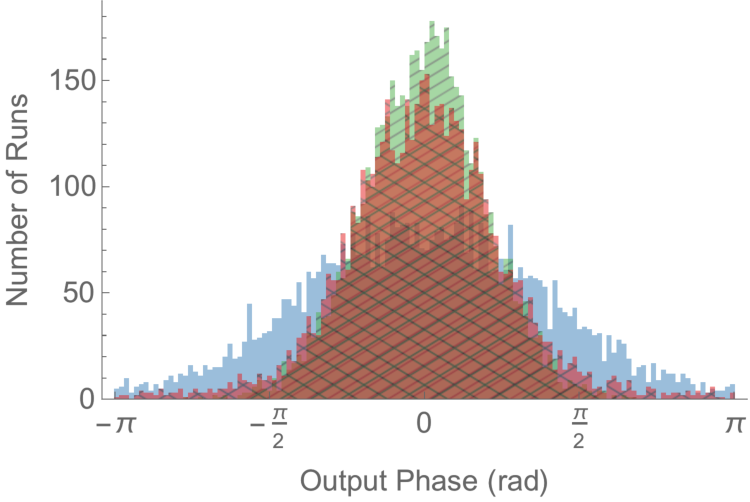
\includegraphics[width=\columnwidth]{totphase1.pdf}}
\caption{Top: Total applied phase over $5000$ runs for no averaging (orange), averaging across the entire system (green) and averaging each phase shifter individually (blue). Bottom: Histogram of the total applied phases. Each individual phase shifter has a variance of $0.1\ \textrm{rad}^{2}$ and each system has $15$ phase shifters in series. The two error averaged circuits are each averaged $4$ times. \label{fig:Total-applied-phase1}}
\end{figure}
%
\begin{figure}
\centerline{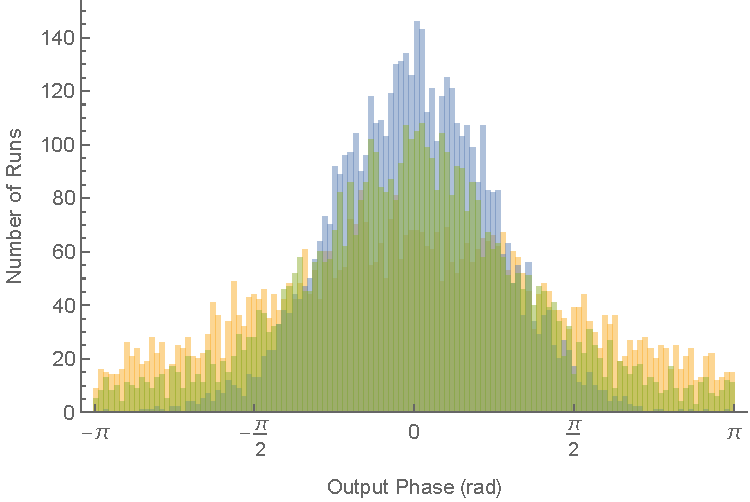
\includegraphics[width=\columnwidth]{totphase2.pdf}}
\caption{Top: Total applied phase over $5000$ runs for no averaging (orange), averaging across the entire system (green) and averaging each phase shifter individually (blue). Bottom: Histogram of the total applied phase. Each individual phase shifter has a variance of $0.3\ \textrm{rad}^{2}$ and each system has $8$ phase shifters in series. The two error averaged circuits are each averaged $4$ times. \label{fig:Total-applied-phase2}}
\end{figure}

The variance of the applied phase was estimated based on the statistical simulation of the total applied phase. Figure~\ref{fig:Variance-in-phase all} shows this variance as a function of $M$, the number of phase shifters in a series. Given the individual applied phases are uncorrelated they are expected to simply add, such that the variance without any Error Averaging is expected to be
\begin{equation}
\textrm{Total Variance}=vM\label{eq:Tot Var no correction}
\end{equation}
where $M$ is the number of phase shifters and $v$ is the variance in the individual phase shifter. The total variance when Error Averaging is similarly expected to be
\begin{equation}
\textrm{Total Variance}=\frac{vM}{N}\label{eq:Tot Var w/ correction}
\end{equation}
where $N$ is the number of times the system is averaged, again $N=1$ implies no averaging. As the phase is an angle with a finite range, this behaviour cannot hold for arbitrarily large $vM$. A completely random phase $\theta$ is still limited by the possible range of values, in our case chosen to be $-\pi<\theta\le\pi$. If the value of $\theta$ is indeed completely random then one will expect a uniform probability distribution of $P\left(\theta\right)=\frac{1}{2\pi}$. This then implies the maximum variance will be given by
\begin{eqnarray}
\textrm{Maximum variance} & = & \int_{-\pi}^{\pi}\theta^{2}P\left(\theta\right)\ d\theta\nonumber \\
& = & \frac{\pi^{2}}{3}\label{eq:Max Var}
\end{eqnarray}

\begin{figure}
\centerline{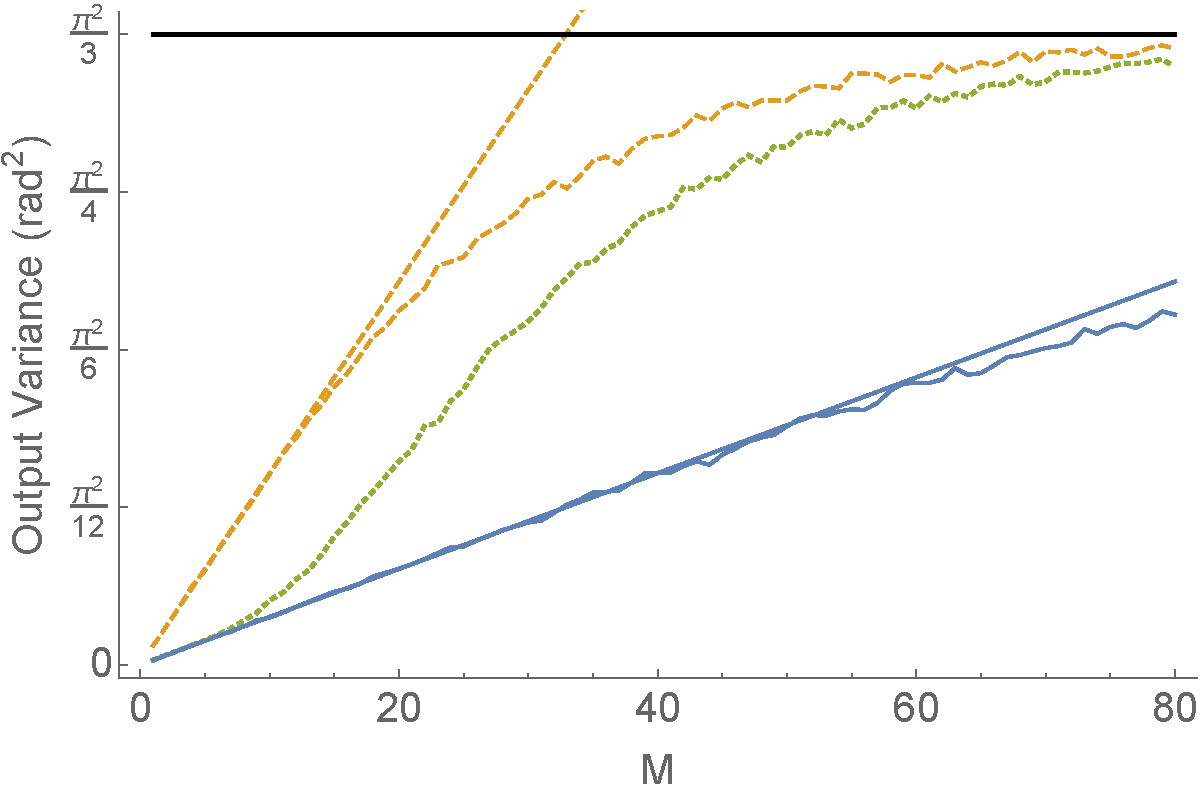
\includegraphics[width=\columnwidth]{phase_all.pdf}}
\caption{Variance in the total applied phase without Error Averaging (orange), when averaging across the entire system (green) and when averaging each component individually (blue), all plotted as a function of the number of phase shifters in series $(M)$. The variance of a single phase shifter is $0.1\ \textrm{rad}^{2}$ and the two error averaged systems averaged 4 times. The predicted, linear variance without any averaging (orange) and with averaging (blue) is also shown. These ignore the fact that the variance is actually the angular variance and so has some maximum allowable value given by Eq. \ref{eq:Max Var}, which is also shown in black. \label{fig:Variance-in-phase all}}
\end{figure}
%
Figure \ref{fig:Variance-in-phase all} shows that the two methods of error correction do indeed initially have the same effect. However the averaging across the system method departs from this linear regime from approximately $M=6$ after which it follows the general form of applying no correction. This suggests there is some limit to the total variation in a system Error Averaging can handle. This is not unexpected due to the limited domain for a phase shift or beam splitter ratio. The fact that averaging across the entire system mirrors the no averaging trend suggest that the positive effects of Error Averaging completely disappear in this regime. Averaging each step however does not appear to fall out of the linear regime. The lower slope at higher total output variance can be attributed to the variance approaching the maximum possible variance.  To determine if and when the averaging each step method of error correction fails, this process was repeated as a function of the variance in a single beam splitter. The total variance was determined from $50000$ data points for each value of $v$. Figure~\ref{fig:Variance(veriance)} demonstrated that again the two error correction methods initially are equivalent. Once more averaging across the system departs from the linear regime and now we can clearly see that so too does the averaging each step.

This is suggestive of the existence of some threshold for the amount of error in a system before Error Averaging fails to be beneficial. A single phase shifter with variance $v_{1}$ is effectively equivalent to $m$ phase shifters with individual variance $v_{2}=\frac{v_{1}}{m}$ if the entire system is being averaged across. This allows the phase error threshold to be estimated at about $0.5\ \textrm{rad}^{2}$ when averaging across each element and $\frac{0.5}{m}\textrm{rad}^{2}$ when averaging across a system of $m$ phase shifters. Explicitly, this suggests a phase variance threshold of $0.5\ \textrm{rad}^{2}$ within the corrected unitary. If each individual beam splitter has a variance of $0.1\ \textrm{rad}^{2}$, averaging across the system would be expected to be in the linear regime when $M\le5$ which is precisely what is seen in Figure \ref{fig:Variance-in-phase all}. These two thresholds obviously do not apply to a general error however it is hoped that with further study might reveal the values for such a threshold.
\begin{figure}
\centerline{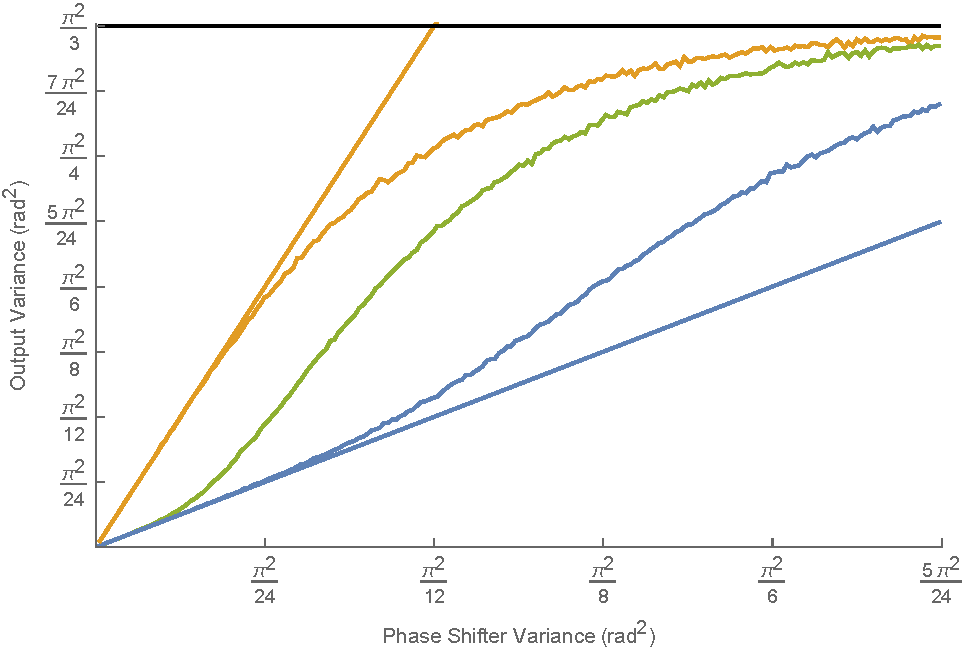
\includegraphics[width=\columnwidth]{variance(variance).pdf}}
\caption{Variance in the total applied phase without Error Averaging (orange), when averaging across the entire system (green) and when averaging each component individually (blue), all plotted as a function of the variance in each individual phase shifter. Each system applied $4$ phase shifters in series, that is $M=4$, and the two error averaged systems averaged $4$ times, that is $N=4$. The predicted variance without any averaging (orange) and with averaging (blue) is also shown along with the maximum allowable variance. \label{fig:Variance(veriance)}}
\end{figure}

It can now be concluded that some hybrid method of Error Averaging would be most suitable in general. The entire system would need to be broken into $x$ smaller systems, which are independently averaged across. The specific value of $x$ would be such that the number of components in the system, $m$, is maximised while the total error within each subsystem is kept below the appropriate threshold.

\section{Four Mode Implementation Comparison \label{Four Mode Impementation Comparison}}

To gain a better understanding of how useful this method of Error Averaging actually is, a more complex system was also investigated along with both methods of redundant error correction. Specifically, a four mode system with four beam splitters, each implemented as above, that is each being its own MZ interferometer as shown in Figure \ref{fig:4 mode basis diagram}. Three different input states were chosen: a single photon input in the top mode and the vacuum state at all other modes$\left(\left|1,0,0,0\right\rangle \right)$, two photons, both in the top mode $\left(\left|2,0,0,0\right\rangle \right)$ and two photons spread across the top two modes $\left(\left|1,1,0,0\right\rangle \right)$. For simplicity the system was chosen to target the identity and error reduction was then applied using both implementations. That is, by averaging each beam splitter as done in section \ref{1 photon N arbitrary} and by concatenating the entire system in an interferometer as shown in Figure \ref{fig: averaging 4 mode diagram}. All results were found using \textit{Mathematica} to sample from the appropriate transformation matrix representing the system and then compute the second order approximation of the photon number expectation values and probabilities for $N=1, 2 \textrm{ and } 4$. All results can be found in Appendix \ref{Appendix full of results}

\begin{figure}[h]
\centerline{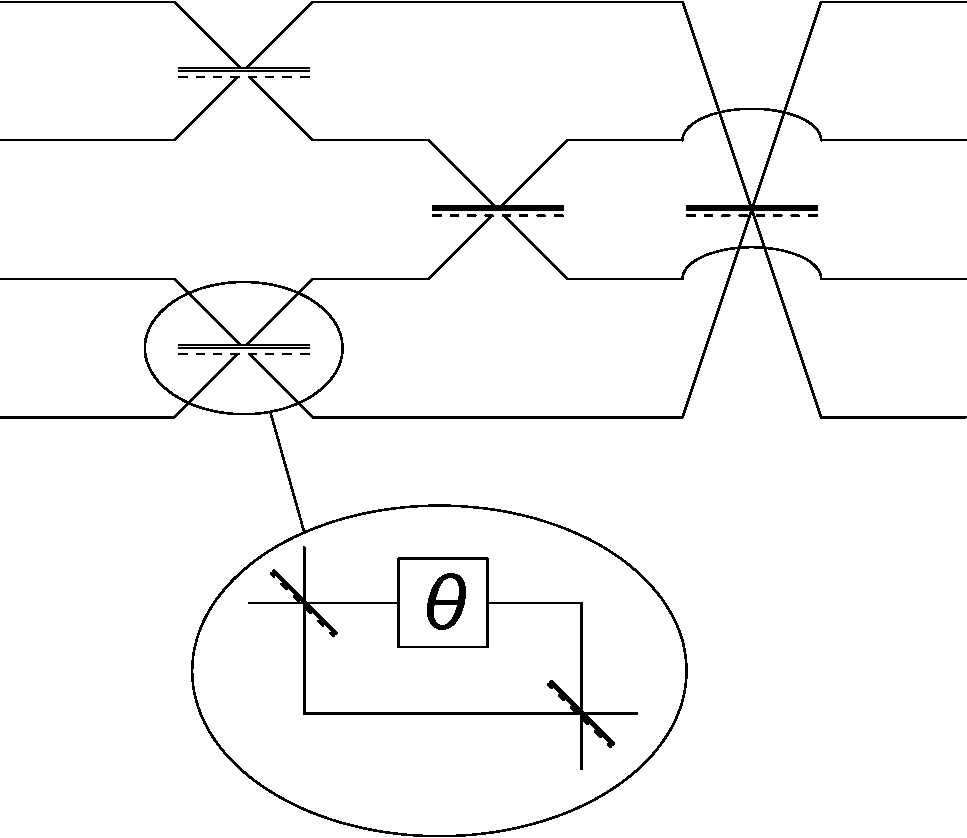
\includegraphics[width=\columnwidth]{4_mode_system.pdf}}
\caption{Diagram of the four mode linear optical network which forms the basis of the four mode set-ups. \label{fig:4 mode basis diagram}}
\end{figure}

\begin{figure}[h]
\centerline{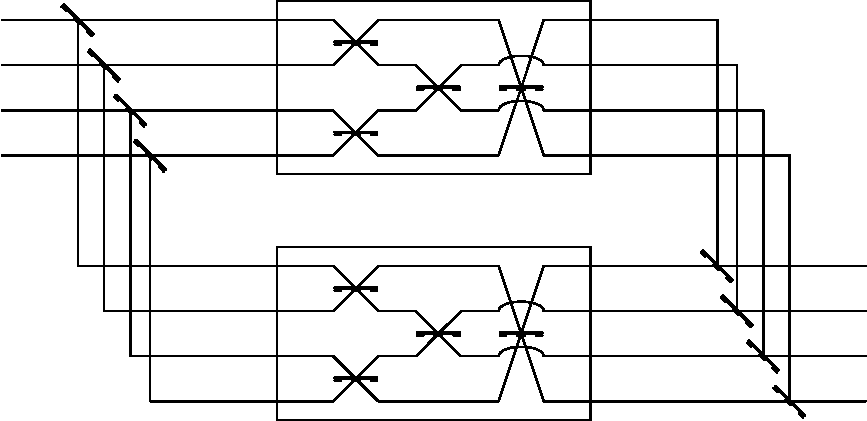
\includegraphics[width=\columnwidth]{4_mode_average_across.pdf}}
\caption{Diagram of the four mode linear optical network averaged across the system once. A two mode system averaged in this fashion could be considered as an Error Averaged dual rail single qubit unitary transformation. \label{fig: averaging 4 mode diagram}}
\end{figure}

These results show that the two correction methods produced equivalent results under the approximations used. The $1/N$ scaling in error after post selection, as seen above, was also observed, suggesting this pattern holds for higher numbers of modes and arbitrary system as expected from Theorem \ref{Theorem 1}.  The analysis that follows is based on the trends observed from these simulations.

\subsubsection{Generalising Example Results}

Starting with no error reduction, and given the correct output state $\left|\psi\right\rangle $ the following sequence can be defined. First defining the probability of obtaining the correct result when $N=1$ takes the form:
\begin{equation}
P_{1}(correct)=1-\frac{a_{1}}{b_{1}}v.
\end{equation}
The probability of an incorrect state is therefore
\begin{equation}
P_{1}(wrong)=\frac{a_{1}}{b_{1}}v.
\end{equation}
At this stage there are no error ports and so $P_{i}(wrong)+P_{i}(correct)$ represents the probability of success as previously defined. Note that the subscript indexes the corresponding number of averaging rounds. Explicitly $i+1$ corresponds to a system with twice as much averaging as $i$.  So, using the same observed form for the probability, averaging once changes these values to:
\begin{eqnarray}
P_{2}(correct) & = & 1-\frac{2a_{1}+1}{2b_{1}}v\nonumber \\
& \equiv & 1-\frac{a_{2}}{b_{2}}v
\end{eqnarray}
\begin{eqnarray}
P_{2}(wrong) & = & \frac{a_{1}}{2b_{1}}v\nonumber \\
& \equiv & \frac{a_{2}}{b_{2}}v
\end{eqnarray}
which can be further iterated.  In general
\begin{eqnarray}
P_{n}(correct) & = & 1-\frac{2a_{n-1}+1}{2b_{n-1}}v\nonumber \\
& = & 1-\frac{\left(2^{n-1}a_{1}+\left(2^{n-1}-1\right)\right)}{2^{n-1}b_{1}}v\\
P_{n}(wrong) & = & \frac{a_{n-1}}{2b_{n-1}}v\nonumber \\
& = & \frac{a_{1}}{2^{n-1}b_{1}}v
\end{eqnarray}
The probability of obtaining the correct state with post selection will then be
\begin{eqnarray}
&  & P_{n}\left(correct\left|\textrm{post selection}\right.\right)\nonumber \\
& = & \left(1-\frac{a_{1}}{2^{n-1}b_{1}}v\right)\xrightarrow[n\rightarrow\infty]{}1\label{eq:PcorrectGeneral}
\end{eqnarray}
The probability of success is 
\begin{equation}
P_{n}\left(success\right) =  1-\frac{\left(2^{n-1}-1\right)\left(a_{1}+1\right)}{2^{n-1}b_{1}}v\nonumber \\
\end{equation}
Hence we get an asympotitic expression for the probability of success to be 
\begin{equation}
\lim_{n\rightarrow\infty}P_{n}\left(success\right)=1-\left(\frac{a_{1}+1}{b_{1}}\right)v\label{eq:PsuccessGeneral}
\end{equation}
The result can be understood to be the first order approximation to Equation \ref{eq:approx commuting, general case}. The $\frac{a_1+1}{b_1}$ coefficient does not quite match what might be expected from Equation \ref{eq:approx commuting, general case} however one might only expect qualitative agreement as there is not any clear isomorphic map between the parameters in the system and the error coefficients of the Lie algebra generators.

This result hints at the self correcting nature of Error Averaging. By considering the inner corrected system with error laden beam splitters as the initial step in the sequence then each further step will be averaging across both the fixed beam splitters and the original error laden system. This could allow some of the beam splitters to be corrected  making the base assumptions on the quality of the fixed beam splitters less restrictive. This is highlighted in Figure \ref{fig:gen system} where, depending on which components are considered to be the system, it is averaged either $8$, $4$ or $2$ times. 

% \section{Scaling of Error Averaging\label{Feasibility section}}
% 
% The previous sections have analysed this protocol in the case of small fixed mode numbers.  We will now discuss the more general situation involving larger numbers of modes.  For these larger systems we are particularly interested in understanding how to minimise the number of encoding resources and while ensuring the system remains in the well understood small error regime of Corollary~\ref{Corollary 2}.
% 
% The number of possible configurations of linear optical elements for a general $m$-mode system is large.  We will therefore consider a constrained set of configurations in the analysis presented here.   We construct the $m$-mode unitary using beam-splitters and phase shifters such that each input mode is connected via some path to each output mode.  Also, these are laid out so that the same number of beam-splitters and phase shifters are encountered by every path. The first requirement ensures that non-trivial interactions occur between all modes.  Note, that even though every mode will be mixed with every other mode, the system is insufficient to implement an arbitrary unitary transformation of the input. The second requirement, that each path has the same number of beam splitters and phase shifters to ensure the system's error profile is completely symmetric.
% 
% To create such a system we choose and even number of modes $m$ arranged in rows. Then we arrange the beam splitters in columns with $b=\frac{m}{2}$ beam splitters in each column. They are arranged such that, starting with the top most mode, the first column mixes nearest neighbour modes, the second column mixes the next nearest neighbour modes and each subsequent column mixes the next closest mode which it is yet to be mixed with as demonstrated in figure \ref{fig:16 mode single photon unitary}. This gives a depth of $c$ columns where $c=\left\lceil \log_{2}(m)\right\rceil $.
% 
% \begin{figure}[h]
% 	\centerline{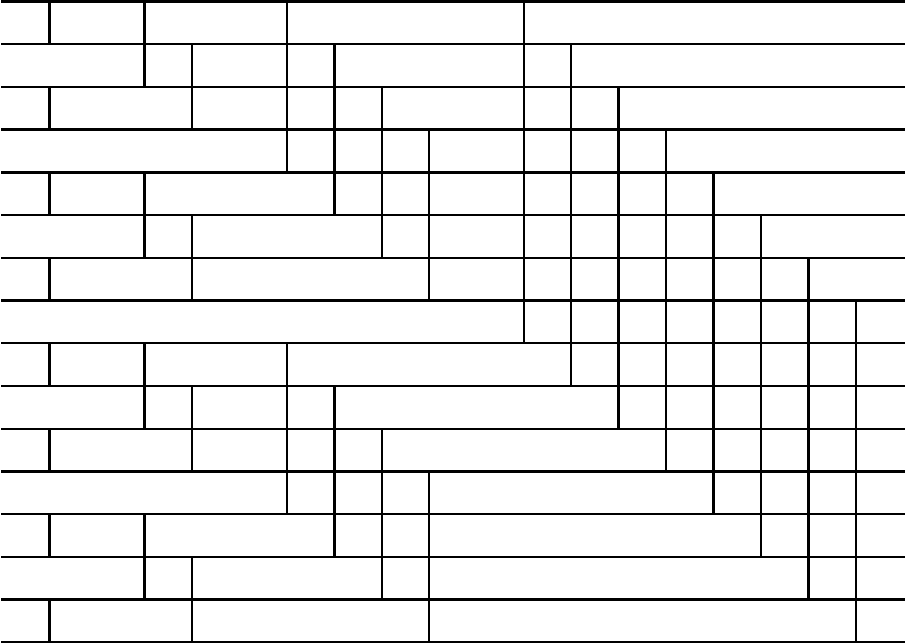
\includegraphics[width=\columnwidth]{16mode_single_photon_unitary.pdf}}
% 	\caption{Example single photon, sixteen mode system. Each vertical line represents a tunable beam splitter which would need to include appropriate phase shifters to improve generality. These were left of . Such a system allows every mode mixed with every other mode in a unique way with equal depth. \label{fig:16 mode single photon unitary}}
% \end{figure}
% 
% As stated above, this arrangement is not suitable for implementing an arbitrary unitary transformation. This is because to $\mathfrak{U\mathrm{(m)}}$ has dimensionality $m^2$ and so one requires a universal decomposition to have at least this many elements with parameters to vary (for such a decomposition see~\cite{reck}). Our arrangement has
% \begin{equation}
% b\times c=\frac{m}{2}\log_{2}(m)
% \end{equation}
% beam-splitters of arbitrary reflectivity and so, the number of free parameters will be only $m\log_{2}(m)$.  However, this arrangement does satisfy the two properties that we required.
% 
% % Do we need this here?
% Using such a system we can either average across the system or average each component individually to protect against errors.
% 
% In the analysis to this point we have made the assumption that perfect, fixed $50:50$ beam splitters can be used to generate the redundancy in the input modes.  
% 
% The following discussion ignores the probability of success of Error Averaging, which will lead to an exponential overhead in the number of times the device must be run before obtaining a successful outcome.  To address this Error Averaging will require a loss recovery code \cite{OQC} however this is outside the scope the current paper. 
% 
% It is worth noting that in the paper \textit{Universal Linear Optics} a single, controllable, beam-splitter was implemented using an tunable Mach-Zehnder interferometer with fidelity $\mathcal{F}=0.992\pm0.008$~\cite{ULO}.
% This suggests that currently it is possible to achieve high quality, low error, tunable linear optics components. 
% 
% One necessary and perhaps sufficient condition for this assumption to be valid is for the number of error causing components in the system to be far greater than the number of perfect components required. This would imply that even if the fixed beam splitters are no better than the variable ones being implemented, Error Averaging will still dramatically reduce the total error in the system.
% 
% %It is known \cite{reck} that a system requires $O\left(m^{2}\right)$ controllable components to be sufficient to implement $\mathfrak{U}\left(m\right)$.
% If such a system is corrected using Error Averaging and the minimum number of correction components then the method of correcting across the entire system would be used. To average a single mode $N$ times, $2\left(N-1\right)$ perfect beam splitters are required. So the precise resource cost will be dependent on the circuits specific set-up. Following on from the previously described set up, we know we can mix $m$ modes in a unique way such that every path has the same number of beam splitters and phase shifters with a circuit depth of $\log_{2}\left(m\right)$.
% 
% Aaronson and Arkhipov, inspired by a boson sampling type system with $n$ photons in the top $n$ modes, have shown \cite{Boson} that for this system to be adequate to implement an arbitrary unitary operation it must be chained together $n$ times. Each block will have $m$ modes, a depth of $\log_{2}\left(m\right)$ and therefore $\frac{m}{2}\log_{2}\left(m\right)$ beam splitters. This then means that our system will have $\frac{mn}{2}\log_{2}\left(m\right)$ error laden components and require a minimum of $2\left(N-1\right)m$ correction components to allow for averaging $N$ times across the entire system. Given that averaging across the entire system falls out of the linear regime very quickly as the depth increases it would likely be insufficient to correct our system. If however each component has Error Averaging applied to it individually then there would need to be at most $mn\log_{2}\left(m\right)\left(N-1\right)$ perfect $50:50$ beam splitters, more than the original size of the circuit. Note this can result in correcting components which cannot possibly be involved in the result. For example if only the top one or two modes have photon inputs then only $2\left(m-1\right)\left(N-1\right)+m\left(n-1\right)\log_{2}\left(m\right)\left(N-1\right)$ correction components are necessary. The upper bound on the number of correction components, $mn\log_{2}\left(m\right)\left(N-1\right)$, is more general, and so will be used for the remainder of this discussion. This suggests something part way between these two cases is necessary. If a system was split up into $x$ sections, each of which is averaged $N$ times, than $2xm\left(N-1\right)$ correction components are necessary. This then gives the very loose inequality of
% \begin{eqnarray}
% 2xm\left(N-1\right) & \ll & \frac{mn}{2}\log_{2}\left(m\right)\nonumber \\
% 4x\left(N-1\right) & \ll & n\log_{2}\left(m\right)\label{eq:veryLooseInequality}
% \end{eqnarray}
% for the assumption that an averaging circuit can be made using relatively perfect beam splitters to be valid. The requirement of Error Averaging to be in the linear regime will also impose the condition that $x\rightarrow n\log_{2}\left(m\right)$ as the error in each component gets bigger. There is the possibility that this is not quite so bad however as most of the perfect beam splitters are actually error averaged themselves as shown in Figure \ref{fig:gen system}. This could allow greater freedom in what is meant by a perfect beam splitter. However even if only the outermost beam splitters are to be considered, and all inner beam splitters are said to be corrected themselves, there will still require between $2m$ and $mn\log_{2}\left(m\right)$ perfect fixed beam splitters.
% 
% Another important issue is to decide how any times the system needs to be averaged, that is, how $N$ needs to grow with $m$ and $n$. It has been shown that for the total systems error to be vanishingly small the error in each individual element in a linear optical system needs to be on the order of $\frac{1}{n}$ where $n$ is the number of photons \cite{arkhipov2014}. It has also been shown that it is necessary for the error to scale as $\frac{1}{n\log_{2}\left(m\right)}$ \cite{Boson} in the case of a boson sampling style system with $1$ photon in the first $n$ modes of an $m$ mode system. Combining these two results gives a necessary scaling of $\frac{1}{n^{2}\log_{2}\left(m\right)}$. All of our results so far suggest the error scales as $\frac{1}{N}$. By using this scaling we can estimate that $N\sim n^{2}\log_{2}\left(m\right)$ for the total error in the output to be preserved. Combining this with Eq. \ref{eq:veryLooseInequality} then gives
% \begin{equation}
% 4x\left(n^{2}\log_{2}\left(m\right)-1\right)\ll n\log_{2}\left(m\right)\label{eq:LooseInequality}
% \end{equation}
% which is clearly not satisfied. This suggests the best hope for the key assumption to be satisfied is if the inner perfect beam splitters are considered to be corrected. As this gives
% \begin{eqnarray}
% 2xm & \ll & \frac{mn}{2}\log_{2}\left(m\right)\nonumber \\
% \implies4x & \ll & n\log_{2}\left(m\right)\label{eq:aBetterInequality}
% \end{eqnarray}
% there is the possibility that this can be satisfied. Even if this is reduced to $4x\approx n\log_{2}\left(m\right)$ there will still be some total reduction in error as the fixed beam splitters are likely to have less total error. It is possible to generalise this result by allowing photons to be inserted into any of the input modes. This will require our system with a depth of $\log_{2}\left(m\right)$ to be chained $m$  times. This can be understood by considering the that an arbitrary unitary transformation requires that a photon from any of the  input modes must be able to interact with all other photons. Given we are using beam splitters as our basic components this limits every interaction to two photon interferences. Each block of depth  will allow any photon to interact with any one other photon and so for a photon to potentially interact with all other photons, we will require $n$ of these blocks. We also need to consider the scaling to allow at least one photon in all $m$ modes giving a scaling of $\frac{1}{mn\log_{2}\left(m\right)}$ to achieve a negligible amount of total error and giving a final rough bound of
% \begin{eqnarray}
% 4x & \ll & m\log_{2}\left(m\right)\label{eq:aDifferentInequality}
% \end{eqnarray}
% where now $x\rightarrow m\log_{2}\left(m\right)$ as the error in each component gets bigger.
% 
% This is, in its current state a unsolved problem. It is hoped that this can be extended to a fault tolerant regime and thresholds can be found so that stronger conclusions on the applicability of Error Averaging can be made.
% 
% \emph{(NOTE: I cannot figure out what the \textbf{key} messages are here.}
% 
% Some thoughts on this section
%
% What this _really_ should be about is the generalisation to $N$ modes.  This wasn't really numerically simulated as it is a bit hard to do that.
% There are some critical problems here that I'm not sure if they are able to be recovered from:
% a) The model of counting for a ``general'' unitary admits that it under counts.
% b) The bit about AA seems _weird_. What does it mean about `n' times!?  AA say nothing about the parametrisation of their problem.  Not sure where this came from.  But an interesting idea is that n-photons into m-modes must have parameters for which there is no sensitivity in the output probability.  
% c) There is a connection to total variation distance (which wasn't actually in AA but in Arkipov's later unitary errors paper), but this isn't actually made.  I think the error model we are talking about won't scale as (n log m)^-1. So I'm thinking the last bit might be wrong.
%
% We are admitting that we aren't looking for fault tolerance here. We really just want to count resources for the generic cases.  I don't think we need to worry about the ``right'' values.  Just count the resources, state the result and then end saying the values needed will depends on how it's used.
%}


\section{Discussion\label{Discussion}}

The analysis presented in~\cref{implementation,averaging at end vs step,Four Mode Impementation Comparison} concentrated on implementing a single-mode phase shift either on it's own or as part of a Mach-Zender interferometer implementing a beam-splitter type transformation.  These could then be further used to build up higher-dimensional unitary transformations using any particular choice of decomposition, for which a specific decomposition was analysed in Section~\ref{Four Mode Impementation Comparison}.

On the other hand, one may want to redundantly encode an entire unitary rather than just the phases defining the internal parameters.  In this case we can use equation~\ref{eq:approx commuting, general case} and for simplicity consider the specific case with $T_l^2= I$
\begin{equation}
	M = U \prod_l e^{-\frac{1}{2}\sigma_l^2} = U e^{-\frac{1}{2} n^2 \sigma^2},
\end{equation}
where the $n^2$ term appears as the product over all $n^2$ generators.
This would result in an effective operator transformation for a $k$ photon state as
\begin{equation}
	\frac{{a^\dagger}_i^{k}}{\sqrt{k!}} \rightarrow 
	e^{-k n^2 \sigma^2/2} \frac{1}{\sqrt{k!}} \left(\sum_j U_{ij} {a^\dagger}_i \right)^k
\end{equation}
The coefficient here represents a reduction in the amplitude should this transformation be applied to a state, and hence represents the probability of success. To achieve a $O(1)$ probability of success, then the operator noise must obey $\sigma = O(k^{-1/2})$ and $\sigma = O(n^{-1})$ as $k,n \rightarrow \infty$.  These results are dependant on the assumptions and the desired performance, in terms of probability of success, will depend on the specific application.  However, it must be kept in mind that no error correction has been performed yet it is still possible to achieve a constant success probability with a reasonable scaling of the noise with respect to the network size. 

Within the constructions presented here some optical elements utilised have been assumed ideal.  In particular, the encoding beam-splitters were assumed to have exactly 50:50 reflectivities.  A more general consideration is that of the fault-tolerance of this encoding.  That is, can the ideal elements be error corrected whilst maintaining the error correcting power of the scheme.   In this paper we have focused on merely the error correcting power of different arrangements of phase shifts and how it varies across two choices of decomposition.  But there will be many and varied choices about how to implement fault tolerant constructions with some better than others, in much the same way as is applicable for discrete system in quantum computing implementations.  Never-the-less, the fact that, under an approximation of small errors the encoding tends to the ideal operation in the limit of large encoding sizes, it would be reasonable to expect that fault-tolerant constructions exist.  

\section{Conclusion\label{Conclusion}}

We have shown how, given multiple noisy copies of a linear optical unitary network, Error Averaging can be use to implement a transformation that tends towards the average with reduced variance at the cost of the probability of success.  After post-selection, Error Averaging forms a rudimentary error correction protocol by filtering the noise from the redundant copies of the unitary network. For this to form a true error correction protocol it will be necessary to introduce some sort of loss correction. The losses which will need to be corrected are unique however in that they are heralded and located, potentially simplifying the problem enormously. The variance in the transformations have been shown to scale as $\frac{1}{N}$ where $N$ represents the number of redundant copies of the network.  We have provided the mathematical basis necessary to determine the effect of Error Averaging on an arbitrary linear unitary and with fully characterised solutions for arbitrary single parameter noise and multiple parameter small Gaussian noise. We have also analytically determined the photon number expectation values for two mode systems with both one and two photon inputs, numerically simulated the output expectation values in four mode systems for both one and two photon inputs and numerically simulated the variance for different arrangements of phase shifters.

Two methods of Error Averaging for phase shifts have been presented which appear to have similar effects under certain conditions. In particular averaging after sequentially applying phases has the same behaviour as averaging each phase provided the errors are small. This behaviour is conjectured to be explained by considering the errors as approximately commuting.

\begin{acknowledgments}
	We thank Michael Bremner for motivating discussions. This research was funded by the Australian Research Council Centre of Excellence for Quantum Computation and Communication Technology (Project No.CE110001027). P.P.R is funded by an ARC Future Fellowship (project FT160100397).
\end{acknowledgments}

\bibliography{references}

\appendix
\begin{widetext}
\section{Four Mode Numerical Results \label{Appendix full of results}}
\FloatBarrier
This appendix contains all simulation results for the four mode system discussed in Section \ref{Four Mode Impementation Comparison}. All results are based on a second order Taylor expansion with $\nu\ll1$.

Tables \ref{tab:1 photon output prob bs} and \ref{tab:1 photon output prob as}
show the output probabilities and correct result probability with
post selection for the single photon input state $\left|1,0,0,0\right\rangle $.
These show that, at least for a single photon the two correction methods
are equivalent. We also see the halving of errors as seen in sections
3.2 and 3.4 suggesting this pattern may hold for a single photon with
an arbitrary number of modes.

\begin{table}
\resizebox{\textwidth}{!}{

\begin{centering}
	\begin{tabular}{|c|c|>{\centering}p{4cm}|>{\centering}p{4cm}|}
		\hline 
		Output State & No Error Reduction & Averaging Beam splitters Once $\left(N=2\right)$ & Averaging Beam splitters Twice $\left(N=4\right)$\tabularnewline
		\hline 
		\hline 
		$\left|1,0,0,0\right\rangle $ & $1-\frac{v}{2}$ & $1-\frac{3v}{4}$ & $1-\frac{7v}{8}$\tabularnewline
		\hline 
		$\left|0,1,0,0\right\rangle $ & $\frac{v}{4}$ & $\frac{v}{8}$ & $\frac{v}{16}$\tabularnewline
		\hline 
		$\left|0,0,1,0\right\rangle $ & $0$ & $0$ & $0$\tabularnewline
		\hline 
		$\left|0,0,0,1\right\rangle $ & $\frac{v}{4}$ & $\frac{v}{8}$ & $\frac{v}{16}$\tabularnewline
		\hline 
		$\left|1,0,0,0\right\rangle $ with post selection & $1-\frac{v}{2}$ & $1-\frac{v}{4}$ & $1-\frac{v}{8}$\tabularnewline
		\hline 
	\end{tabular}
	\par\end{centering}

}

\caption[Output probabilities for various levels of correcting the individual
beam splitters in a 4 mode set-up given an input of the state $\left|1,0,0,0\right\rangle $
.]{Output probabilities for various levels of correcting the individual
beam splitters in a 4 mode set-up given an input of the state $\left|1,0,0,0\right\rangle $
where $v$ is the variance of the phase error . \label{tab:1 photon output prob bs}}
\end{table}
\begin{table}
\resizebox{\textwidth}{!}{

\begin{centering}
	\begin{tabular}{|c|c|>{\centering}p{4cm}|>{\centering}p{4cm}|}
		\hline 
		Output State & No Error Reduction & Averaging Across the System Once $\left(N=2\right)$ & Averaging Across the System Twice $\left(N=4\right)$\tabularnewline
		\hline 
		\hline 
		$\left|1,0,0,0\right\rangle $ & $1-\frac{v}{2}$ & $1-\frac{3v}{4}$ & $1-\frac{7v}{8}$\tabularnewline
		\hline 
		$\left|0,1,0,0\right\rangle $ & $\frac{v}{4}$ & $\frac{v}{8}$ & $\frac{v}{16}$\tabularnewline
		\hline 
		$\left|0,0,1,0\right\rangle $ & $0$ & $0$ & $0$\tabularnewline
		\hline 
		$\left|0,0,0,1\right\rangle $ & $\frac{v}{4}$ & $\frac{v}{8}$ & $\frac{v}{16}$\tabularnewline
		\hline 
		$\left|1,0,0,0\right\rangle $ with post selection & $1-\frac{v}{2}$ & $1-\frac{v}{4}$ & $1-\frac{v}{8}$\tabularnewline
		\hline 
	\end{tabular}
	\par\end{centering}

}

\caption[Output probabilities for various levels of correcting the across the
system in a 4 mode set-up given an input of the state $\left|1,0,0,0\right\rangle $.]{Output probabilities for various levels of correcting the across
the system in a 4 mode set-up given an input of the state $\left|1,0,0,0\right\rangle $
where $v$ is the variance of the phase error. \label{tab:1 photon output prob as}}
\end{table}


Tables \ref{tab:2 photon output prob bs} and \ref{tab:2 photon output prob as}
show the output probabilities and correct result probability with
post selection for the single photon input state $\left|2,0,0,0\right\rangle $.
What we see is, unsurprisingly, much the same as in the single photon
case with a heightened susceptibility to the error. This includes
the halving pattern however this is expected as adding two photons
in the same mode will not necessarily lead to new interference effects
being observed.

\begin{table}
\resizebox{\textwidth}{!}{

\begin{centering}
	\begin{tabular}{|c|>{\centering}p{4cm}|>{\centering}p{4cm}|}
		\hline 
		Output State & No Error Reduction & Averaging Beam splitters Once $\left(N=2\right)$\tabularnewline
		\hline 
		\hline 
		$\left|2,0,0,0\right\rangle $ & $1-v$ & $1-\frac{3v}{2}$\tabularnewline
		\hline 
		$\left|0,2,0,0\right\rangle $ & $0$ & $0$\tabularnewline
		\hline 
		$\left|0,0,2,0\right\rangle $ & $0$ & $0$\tabularnewline
		\hline 
		$\left|0,0,0,2\right\rangle $ & $0$ & $0$\tabularnewline
		\hline 
		$\left|1,1,0,0\right\rangle $ & $\frac{v}{2}$ & $\frac{v}{4}$\tabularnewline
		\hline 
		$\left|1,0,1,0\right\rangle $ & $0$ & $0$\tabularnewline
		\hline 
		$\left|1,0,0,1\right\rangle $ & $\frac{v}{2}$ & $\frac{v}{4}$\tabularnewline
		\hline 
		$\left|0,1,1,0\right\rangle $ & $0$ & $0$\tabularnewline
		\hline 
		$\left|0,1,0,1\right\rangle $ & $0$ & $0$\tabularnewline
		\hline 
		$\left|0,0,1,1\right\rangle $ & $0$ & $0$\tabularnewline
		\hline 
		$\left|2,0,0,0\right\rangle $ with post selection & $1-v$ & $1-\frac{v}{2}$\tabularnewline
		\hline 
	\end{tabular}
	\par\end{centering}

}

\caption[Output probabilities for various levels of correcting the individual
beam splitters in a 4 mode set-up given an input of the state $\left|2,0,0,0\right\rangle $.]{Output probabilities for various levels of correcting the individual
beam splitters in a 4 mode set-up given an input of the state $\left|2,0,0,0\right\rangle $
where $v$ is the variance of the phase error. \label{tab:2 photon output prob bs}}
\end{table}
\begin{table}
\resizebox{\textwidth}{!}{

\begin{centering}
	\begin{tabular}{|c|>{\centering}p{4cm}|>{\centering}p{4cm}|>{\centering}p{4cm}|}
		\hline 
		Output State & No Error Reduction & Averaging Beam splitters Once $\left(N=2\right)$ & Averaging Beam splitters Twice $\left(N=4\right)$\tabularnewline
		\hline 
		\hline 
		$\left|2,0,0,0\right\rangle $ & $1-v$ & $1-\frac{3v}{2}$ & $1-\frac{7v}{4}$\tabularnewline
		\hline 
		$\left|0,2,0,0\right\rangle $ & $0$ & $0$ & $0$\tabularnewline
		\hline 
		$\left|0,0,2,0\right\rangle $ & $0$ & $0$ & $0$\tabularnewline
		\hline 
		$\left|0,0,0,2\right\rangle $ & $0$ & $0$ & $0$\tabularnewline
		\hline 
		$\left|1,1,0,0\right\rangle $ & $\frac{v}{2}$ & $\frac{v}{4}$ & $\frac{v}{8}$\tabularnewline
		\hline 
		$\left|1,0,1,0\right\rangle $ & $0$ & $0$ & $0$\tabularnewline
		\hline 
		$\left|1,0,0,1\right\rangle $ & $\frac{v}{2}$ & $\frac{v}{4}$ & $\frac{v}{8}$\tabularnewline
		\hline 
		$\left|0,1,1,0\right\rangle $ & $0$ & $0$ & $0$\tabularnewline
		\hline 
		$\left|0,1,0,1\right\rangle $ & $0$ & $0$ & $0$\tabularnewline
		\hline 
		$\left|0,0,1,1\right\rangle $ & $0$ & $0$ & $0$\tabularnewline
		\hline 
		$\left|2,0,0,0\right\rangle $ with post selection & $1-v$ & $1-\frac{v}{2}$ & $1-\frac{v}{4}$\tabularnewline
		\hline 
	\end{tabular}
	\par\end{centering}

}

\caption[Output probabilities for various levels of correcting the across the
system in a 4 mode set-up given an input of the state $\left|2,0,0,0\right\rangle $.]{Output probabilities for various levels of correcting the across
the system in a 4 mode set-up given an input of the state $\left|2,0,0,0\right\rangle $
where $v$ is the variance of the phase error. \label{tab:2 photon output prob as}}
\end{table}


Tables \ref{tab:1,1 photon output prob as} and \ref{tab:1,1 photon output prob as}
show the output probabilities and correct result probability with
post selection for the single photon input state $\left|1,1,0,0\right\rangle $.
It can once more be seen that the two methods of error correction
appear to be equivalent. Now there is an underlying pattern clearly
forming which appears to hold for arbitrary one and two photon inputs.
This is important as it allows us to conclude about when it is most
useful to use each type of correction. It also allowed a prediction
of the error models for applications of Error Averaging, as discussed
below.

\begin{table}
\resizebox{\textwidth}{!}{

\begin{centering}
	\begin{tabular}{|c|>{\centering}p{4cm}|>{\centering}p{4cm}|>{\centering}p{4cm}|}
		\hline 
		Output State & No Error Reduction & Averaging Beam splitters Once $\left(N=2\right)$ & Averaging Beam splitters Twice $\left(N=4\right)$\tabularnewline
		\hline 
		\hline 
		$\left|2,0,0,0\right\rangle $ & $\frac{v}{2}$ & $\frac{v}{4}$ & $\frac{v}{8}$\tabularnewline
		\hline 
		$\left|0,2,0,0\right\rangle $ & $\frac{v}{2}$ & $\frac{v}{4}$ & $\frac{v}{8}$\tabularnewline
		\hline 
		$\left|0,0,2,0\right\rangle $ & $0$ & $0$ & $0$\tabularnewline
		\hline 
		$\left|0,0,0,2\right\rangle $ & $0$ & $0$ & $0$\tabularnewline
		\hline 
		$\left|1,1,0,0\right\rangle $ & $1-\frac{3v}{2}$ & $1-\frac{7v}{4}$ & $1-\frac{15v}{8}$\tabularnewline
		\hline 
		$\left|1,0,1,0\right\rangle $ & $\frac{v}{2}$ & $\frac{v}{8}$ & $\frac{v}{16}$\tabularnewline
		\hline 
		$\left|1,0,0,1\right\rangle $ & $0$ & $0$ & $0$\tabularnewline
		\hline 
		$\left|0,1,1,0\right\rangle $ & $0$ & $0$ & $0$\tabularnewline
		\hline 
		$\left|0,1,0,1\right\rangle $ & $\frac{v}{2}$ & $\frac{v}{8}$ & $\frac{v}{16}$\tabularnewline
		\hline 
		$\left|0,0,1,1\right\rangle $ & $0$ & $0$ & $0$\tabularnewline
		\hline 
		$\left|1,1,0,0\right\rangle $ with post selection & $1-\frac{3v}{2}$ & $1-\frac{3v}{4}$ & $1-\frac{3v}{8}$\tabularnewline
		\hline 
	\end{tabular}
	\par\end{centering}

}

\caption[Output probabilities for various levels of correcting the individual
beam splitters in a 4 mode set-up given an input of the state $\left|1,1,0,0\right\rangle $.]{Output probabilities for various levels of correcting the individual
beam splitters in a 4 mode set-up given an input of the state $\left|1,1,0,0\right\rangle $
where $v$ is the variance of the phase error. \label{tab:1,1 photon output prob bs}}
\end{table}
\begin{table}
\resizebox{\textwidth}{!}{

\begin{centering}
	\begin{tabular}{|c|>{\centering}p{4cm}|>{\centering}p{4cm}|>{\centering}p{4cm}|}
		\hline 
		Output State & No Error Reduction & Averaging Beam splitters Once $\left(N=2\right)$ & Averaging Beam splitters Twice $\left(N=4\right)$\tabularnewline
		\hline 
		\hline 
		$\left|2,0,0,0\right\rangle $ & $\frac{v}{2}$ & $\frac{v}{4}$ & $\frac{v}{8}$\tabularnewline
		\hline 
		$\left|0,2,0,0\right\rangle $ & $\frac{v}{2}$ & $\frac{v}{4}$ & $\frac{v}{8}$\tabularnewline
		\hline 
		$\left|0,0,2,0\right\rangle $ & $0$ & $0$ & $0$\tabularnewline
		\hline 
		$\left|0,0,0,2\right\rangle $ & $0$ & $0$ & $0$\tabularnewline
		\hline 
		$\left|1,1,0,0\right\rangle $ & $1-\frac{3v}{2}$ & $1-\frac{7v}{4}$ & $1-\frac{15v}{8}$\tabularnewline
		\hline 
		$\left|1,0,1,0\right\rangle $ & $\frac{v}{2}$ & $\frac{v}{8}$ & $\frac{v}{16}$\tabularnewline
		\hline 
		$\left|1,0,0,1\right\rangle $ & $0$ & $0$ & $0$\tabularnewline
		\hline 
		$\left|0,1,1,0\right\rangle $ & $0$ & $0$ & $0$\tabularnewline
		\hline 
		$\left|0,1,0,1\right\rangle $ & $\frac{v}{2}$ & $\frac{v}{8}$ & $\frac{v}{16}$\tabularnewline
		\hline 
		$\left|0,0,1,1\right\rangle $ & $0$ & $0$ & $0$\tabularnewline
		\hline 
		$\left|1,1,0,0\right\rangle $ with post selection & $1-\frac{3v}{2}$ & $1-\frac{3v}{4}$ & $1-\frac{3v}{8}$\tabularnewline
		\hline 
	\end{tabular}
	\par\end{centering}

}

\caption[Output probabilities for various levels of correcting the across the
system in a 4 mode set-up given an input of the state $\left|1,1,0,0\right\rangle $.]{Output probabilities for various levels of correcting the across
the system in a 4 mode set-up given an input of the state $\left|1,1,0,0\right\rangle $
where $v$ is the variance of the phase error. \label{tab:1,1 photon output prob as}}
\end{table}
\end{widetext}
\end{document}
%
% If in two-column mode, this environment will change to single-column
% format so that long equations can be displayed. Use
% sparingly.
%\begin{widetext}
% put long equation here
%\end{widetext}

% figures should be put into the text as floats.
% Use the graphics or graphicx packages (distributed with LaTeX2e)
% and the \includegraphics macro defined in those packages.
% See the LaTeX Graphics Companion by Michel Goosens, Sebastian Rahtz,
% and Frank Mittelbach for instance.
%
% Here is an example of the general form of a figure:
% Fill in the caption in the braces of the \caption{} command. Put the label
% that you will use with \ref{} command in the braces of the \label{} command.
% Use the figure* environment if the figure should span across the
% entire page. There is no need to do explicit centering.

% \begin{figure}
% \includegraphics{}%
% \caption{\label{}}
% \end{figure}

% Surround figure environment with turnpage environment for landscape
% figure
% \begin{turnpage}
% \begin{figure}
% \includegraphics{}%
% \caption{\label{}}
% \end{figure}
% \end{turnpage}

% tables should appear as floats within the text
%
% Here is an example of the general form of a table:
% Fill in the caption in the braces of the \caption{} command. Put the label
% that you will use with \ref{} command in the braces of the \label{} command.
% Insert the column specifiers (l, r, c, d, etc.) in the empty braces of the
% \begin{tabular}{} command.
% The ruledtabular enviroment adds doubled rules to table and sets a
% reasonable default table settings.
% Use the table* environment to get a full-width table in two-column
% Add \usepackage{longtable} and the longtable (or longtable*}
% environment for nicely formatted long tables. Or use the the [H]
% placement option to break a long table (with less control than 
% in longtable).
% \begin{table}%[H] add [H] placement to break table across pages
% \caption{\label{}}
% \begin{ruledtabular}
% \begin{tabular}{}
% Lines of table here ending with \\
% \end{tabular}
% \end{ruledtabular}
% \end{table}

% Surround table environment with turnpage environment for landscape
% table
% \begin{turnpage}
% \begin{table}
% \caption{\label{}}
% \begin{ruledtabular}
% \begin{tabular}{}
% \end{tabular}
% \end{ruledtabular}
% \end{table}
% \end{turnpage}

% Specify following sections are appendices. Use \appendix* if there
% only one appendix.
%\appendix
%\section{}

% If you have acknowledgments, this puts in the proper section head.
%\begin{acknowledgments}
% put your acknowledgments here.
%\end{acknowledgments}
% ****** End of file apstemplate.tex ******
% vim: nofoldenable linebreak tw=0 
